\documentclass{../tech_reports/template/llncs}
%
\usepackage{url}
\usepackage{amsmath} % use equations
\usepackage{amssymb} % Let Sun have a black triangle
\usepackage{graphicx} % allow PNGs as graphics
\usepackage{epstopdf} % Call epstopdf "on the fly"
\usepackage{tabularx} % adds X alignment and allows \textwidth width for tables
\def\arraystretch{1.5} % add some padding to table cells
\usepackage[labelfont=bf]{caption} % bold labels for Table, Figure etc.
\RequirePackage[utf8]{inputenc} % support Umlauts and special characters
\usepackage{microtype} % use space more efficiently and hyphenate smarter: all in all looks a lot sexier
\newcommand\blfootnote[1]{%
    \begingroup
    \renewcommand\thefootnote{}\footnote{#1}%
    \addtocounter{footnote}{-1}%
    \endgroup
}
\usepackage{listings} % allow source code environment
\lstset{ % make tildes readable in lstlistings
      literate={~} {$\sim$}{1}
}
\lstdefinestyle{flux} { % custom syntax highlighting for FLUX
  frame=L,
  xleftmargin=\parindent,
  basicstyle=\footnotesize\ttfamily,
  breakatwhitespace=true,
  numbers=left,
  escapechar=\%,
  numberstyle=\tiny,
  numberblanklines=false,
  captionpos=b,
  emph={perform, poss, state\_update, main\_loop, init},
  emphstyle=\textbf,
}
\lstset{style=flux} % activate flux syntax highlighting in listings
\usepackage[detect-all,round-mode=places]{siunitx} % A comprehensive (SI) units package
\usepackage{latexsym} % allows special symbols
\usepackage{graphicx} % enables figures
\usepackage{caption} % Support for captions
\usepackage{subcaption} % Support for sub-captions
\usepackage{csquotes} % Context sensitive quotation facilities
\usepackage{booktabs} % Publication quality tables in LaTeX
\usepackage{todonotes} % Mark­ing things to do in a LaTeX doc­u­ment
\usepackage[backend=biber,url=false]{biblatex} % Bibliographies in LaTeX using BibTeX for sorting only
\addbibresource{content/sources.bib}
\usepackage[pdfdisplaydoctitle,linkcolor=theblue,citecolor=theblue,urlcolor=thered]{hyperref} % Extensive support for hypertext in LaTeX (load last)
\RequirePackage[hyphenbreaks]{breakurl} % allow hyphenation in URLs
\usepackage{cleveref} % Intelligent cross-referencing, load after hyperref
% Make autoref talk about lines in lstlistings:
\def\lstnumberautorefname{Line}
% Make autoref start (sub-(sub-))sections with a capital S
\def\sectionautorefname{Section}
\def\subsectionautorefname{Section}
\def\subsubsectionautorefname{Section}
% Fancy headers and footers to add the page number:
\makeatletter
\providecommand\phantomcaption{\caption@refstepcounter\@captype}
\makeatother
\usepackage{fancyhdr}
\pagestyle{fancy}
\fancyhf{
  \fancyhead[L]{\rightmark}
  \fancyhead[R]{\thepage}
}
%
\title{Research Lab \enquote{Multi-Agent Programming Contest 2014}}
\subtitle{Final Report}
%\titlerunning{logprog}
\author{Artur Daudrich$^{\star}$ \and Sergey Dedukh$^{\diamond}$ \and Manuel Mittler$^{\odot}$ \and Michael Ruster$^{\circ}$ \and Michael Sewell$^{\dagger}$ \and Yuan Sun$^{\blacktriangle}$\blfootnote{The symbols after the authors' names indicate who wrote which section. When there are multiple symbols, it means that the first part of author(s) wrote it and the second part significantly corrected/updated and proofread it. E.g. $^{\star/\odot,\dagger/\blacktriangle}$ would indicate $^{\star}$ and $^{\odot}$ are the authors and $^{\dagger}$ and $^{\blacktriangle}$ corrected it.}}
\institute{University of Koblenz-Landau, Campus Koblenz}
%
\newcommand{\mars}{\enquote{Agents on Mars}}
\begin{document}
\maketitle
\pagenumbering{roman}
\tableofcontents
\clearpage
\pagenumbering{arabic}

\section[Motivation and Background]{Motivation and Background$^\dagger$}
\todo{The subsections are quite short. We probably should merge them later on. Also, we'll have to take a look of just about how much we want to talk about the MAPC Mars scenario at this point already. If we keep it as general as we currently are, this will probably be fine. Within the fundamentals part, we can then talk about agents, actions, roles, attributes, what is a zone and so forth.}
\section{Motivation and background$^\dagger$}
\label{alg:zon_calculation}
The \emph{Multi-Agent Programming Contest} is an annual online programming contest hosted by the Clausthal University of Technology since 2005.
Participation is free to any interested groups.
There are no monetary rewards for the winning groups.
The aim of the MAPC is to promote academic interest in the field  of multi-agent systems, that is, systems in which multiple artificial agents have to collaborate to achieve a goal.

The nature of the task in which the agents compete in the MAPC has changed over the years, but since 2011 it has been the same \enquote{Agents on Mars} scenario, which will be described below.
The winner and further rankings of each year's contest are determined by having each group's agent face off against the other in a tournament, and awarding points to each team according to their performance in each match.

\subsection{The \enquote{Agents on Mars} scenario$^\dagger$}
The \enquote{Agents on Mars} scenario is the one that has been used in the yearly MAPC since 2011.
In it, two opposing teams of agents are placed on nodes in a randomized graph.
Each node in the graph has a value which is used for scoring, and agents can traverse the graph by moving along the edges connecting the nodes.
The \enquote{Agents on Mars} name relates to the fictional background \enquote{story} of the scenario: Man has populated Mars, and must find and occupy wells of water on the surface of the planet and protect them from \enquote{pirates}.

The simulation is turn-based, and each agent can perform one action per turn.
There are 28 agents in each team, and each agent belongs to one of five different agent classes, and the agent's type determines the kind of actions the agent can perform and other values used to further differentiate agent classes.
The goal of each match is to have a higher score than the opponent's team at the end of a predetermined number of steps (400 in the 2014 MAPC).
A high score is achieved by finding localized parts of the graph which contain high-value nodes, surrounding these \enquote{zones} with one's own agents, and protecting them from enemy agents' attacks.
The full background story, as well as the more detailed official description of the scenario, can be found in the scenario description provided by the MAPC organizers~\cite{ahlbrecht_mapc_2014}.

\subsection{The \emph{MAKo} (Multi-Agents Koblenz) team$^\dagger$}
The German University of Koblenz-Landau participated in the 2014 MAPC with a small team of graduate students in the scope of a research lab.
The students who participated in research lab until its end were Artur Daudrich, Sergey Dedukh, Manuel Mittler, Michael Ruster, Michael Sewell and Yuan Sun.
The research lab consisted of an initial seminar phase and the longer project phase, where the students designed and implemented the multi-agent architecture used to participate in the MAPC.

\section{Scientific Background and Fundamentals}
\subsection{MAPC: Contest and Scenario}
\todo{Write this section}
What is the general scenario? Agents on mars trying to find water in a competitive manner against another team. Explain the concept of zones, gaining points, achievements and also how agents differ from each other. Introduce the notion of \emph{zoning} as the process of finding and forming a zone (including upkeeping by defense?).
I've put this section first so the later chapters can already rely on the reader knowing what the scenario is about. Furthermore, we can then directly rule out concepts which we are presenting by applying them theoretically onto the scenario/our needs.

\subsection{Agent Programming Concepts}
\todo{Write this section}
\subsubsection[BDI.]{BDI$^\blacktriangle$}
\subsubsection[BDI]{BDI$^{\blacktriangle,\diamond}$}\label{fun:BDI}
Using cognitive modelling techniques for agent development enable autonomous behaviour and reasoning for automated problem solving.
This also allows the analysis of real world behaviour through simulations with agents.
Problems can hence be automatically solved through self-organised groups of agents and new knowledge can be drawn from such simulations.
The beliefs, desires and intentions (short: \emph{BDI}) model, is a widespread software model for developing intelligent agents situated in complex and dynamic environments.
There, the basic characteristics of an agents' mental state are expressed through beliefs, desires and intentions which are explained in more detail later in this section.
The BDI logic system is quite easy to implement in software agents and to some extent promises human-like reasoning behaviour.
Hence, it has been widely used in the field of artificial intelligence in computer science.
This section begins with the roots of the BDI model by mentioning the scientific papers that led to it.
It then continues with an explanation of practical reasoning after which the components of the BDI model are presented in greater detail.
% TODO if there is more to come, I will add it here. I still haven't made it through this text.

In 1987, Bratman~\cite{MICHAEL_PlansResource_1988} discussed the relationship between beliefs, desires, intentions and actions as well their roles in agent behaviours.
This can be seen as the introduction of the BDI model which was revised in 1991 by Rao and Georgeff~\cite{rao_modeling_1991}.
They formalised the model to a first order logic and treated beliefs, desires and intentions as three modal operators while giving intentions equal importance compared to beliefs and desires.
Rao and Georgeff then continued to apply this theoretical foundation to concrete BDI agents, applying them in an airline traffic management application~\cite{Rao_BDITheory_1995}.
Nowadays, BDI agents are deployed in high technology industrial areas such as fault diagnosis on space shuttles, but also in commercial fields and entertainment such as robot soccer games.

The BDI model has its roots in philosophy as found in Bratman's theory of practical reasoning~\cite{Sebastian_Hierarchical_2006}.
Practical reasoning involves two important processes: deciding what goals should be achieved, and how they should be achieved.
The former process is known as \emph{deliberation}, the latter as \emph{means-ends reasoning}~\cite{Gerhard_MultiSystem_1999}.
Means-ends reasoning is a method to make plans for achieving goals based on current states.
The idea of means-ends reasoning is to reduce the difference between the current state and a goal, furthermore, the method is applied recursively.
When an agent is placed in an environment, it should autonomously decide what to do and how to do it.
In general, an agent could execute many different actions but maybe only a few of them would have a desired effect on the environment.
Various external properties can have influence on the feasibility of achieving the agent's goals\todo{\textbf{@yuansun1990}: this part confused me a bit. I don't think, \enquote{affairs} was the right word here. Please check if I still understood what you wanted to say.}.
The deliberation process filters what options are actually possible in the current state.
It then determines which of these options will become intentions.
For example, if you are thirsty and standing in a supermarket, then you might be faced with the decision to choose a drink.
There can be a lot of options like wine, beer, water, lemonade or juice.
However, picking up a bottle of wine or beer is not allowed in Germany for people under the age of 16. % Germany, sadly a proud nation of drunkards.
After collecting all the available options, you must choose and commit to some of them which become intentions next.
Subsequently, we need the mean-ends reasoning process to plan how to achieve these intentions.
If your intention is to buy a bottle of water, you may then plan to go to the shelf with water on it, reach for such a bottle, take it to the checkout counter and pay for it.
Finally, you have to execute this plan to buy the bottle of water.

The BDI model, as an applicable theory of practical reasoning, consists of three components which are beliefs, desires and intentions.
These are subsequently explained each.

Beliefs represent the informational state of the agent~\cite{Rao_BDITheory_1995} and are updated appropriately after each sensing action.
They may be implemented as a variable, a database, a set of logical expressions or some other data structure~\cite{Rao_BDITheory_1995}.
Beliefs model the agent's look at the world.
They can express information about the environment, other agents or the agent itself.
An agent may update its beliefs at any time.
Agents receive new information from the perception of the environment and the execution of intentions.
An agent can use sensors to perceive the environment and store their output as beliefs.
Beliefs are not the same concept as knowledge.
Knowledge is the realisation of a fact whereas a belief models \enquote{knowledge} which is believed by the agent.
Beliefs do not necessarily have to be true from a global perspective.
But from the agent's perspective, they are.
Hence, beliefs can be seen as local knowledge.
Likewise, beliefs can be global knowledge when they are true in a global sense.

Desires represent the motivational state of the agent~\cite{Rao_BDITheory_1995}.
In other words, desires represent objectives or situations that the agent would like to accomplish or bring about.
Desires can be but do not need to be achieved.
% Although similar, desires can be distinguished from goals.
Multiple desires can be inconsistent with each other and the agent does not need to know the means of achieving these desires.
They are inputs to the agent's deliberation process, which results in the agent choosing a subset of desires that are both consistent and achievable.
Such consistent and achievable desires are usually called \emph{goals}~\cite{Gerhard_MultiSystem_1999}.
For example, sleeping and working may be both one's desires, but they can not both be one's goals at the same time because they conflict with each other.

Intentions are desires or actions that an agent committed itself to achieve~\cite{Alejandro_LearnBDI_2004}.
Their meaning is stronger than that of desires.
Desires are merely wishes that may be achieved or may be not, but intentions are decided to be achieved to a reasonable extent.
Michael Wooldridge~\cite{Gerhard_MultiSystem_1999} concluded four functions of intentions in practical reasoning:
\begin{itemize}
  \item Intentions driving means-ends reasoning means that intentions have decisive influences on the actions which the agent will execute.
    Agents are expected to determine ways of achieving intentions.
  \item Intentions constrain future deliberation.
    This means that options which would be in conflict with an already chosen intention will not be considered.
  \item Intentions persist means that intentions will not be given up unless there is a rational reason to do so.
    This is important because if an agent immediately dropped its intentions without devoting resources to achieving them, it will never achieve anything~\cite{Gerhard_MultiSystem_1999}.
    Hence, intentions are committed desires which can not be easily abandoned.
    A reason to drop an intention nevertheless could be e.g. when an external event made the intention impossible or a lot more difficult to achieve.
  \item Intentions influence beliefs upon which future practical reasoning is based.
    This expresses that an intention is believed to be eventually achieved under \enquote{normal circumstances}.
    Practically, after deciding on an intention, the agent will add the intention as a belief.
    This allows the agent to plan for the future on the assumption that the intention will be achieved.
\end{itemize}
Intentions play an important role in the BDI model as they lead to actions and influence future beliefs and intention selection.

Beliefs, desires and intentions are the foundation of BDI agents.
Yet, further components are needed to build the connection between these three components and thereby implement BDI agents.
Naturally, the architecture of BDI agents differs in detail depending on their tasks.
However, they all share a core architecture which is depicted in \autoref{fig:bdi_architecture}.
Its components are explained in the following paragraphs.
% TODO we will have to place this somewhere else as it contains elements like BRF which are explained waaay later.
\begin{figure}[htbp]
  \centering
  \includegraphics[width=\textwidth]{images/BDIAr}
  \caption{Brief BDI architecture~\cite{BDIA}}
  \label{fig:bdi_architecture}
\end{figure}

The sensors of a BDI agent perceive the environment and convert the perceptions to signals as inputs for the belief revision function (short: \emph{BRF}).
This function collects the external perceptions as well as the beliefs which are already stored in the beliefs.
It then processes the information and updates the beliefs accordingly.
The belief revision function prefers minimal change over modifying a lot and hence tries to preserve as much information as possible~\cite{Antje_SpatialBelief_2011}.
While processing the new and old information, the BRF will also solves inconsistencies, e.g.\ when an agent perceives information which contradicts a belief it has.

The belief set's data may be modelled as sentences, rules or some other manifestations.
In the \emph{AGM approach} (named after their proponents, Alchourrón, Gärdenfors, and Makinson)~\cite{alchourron_revision_1985}, an agent's beliefs are modeled by a deductively closed set of formulas called a \emph{beliefs set}~\cite{James_revise_2011}. 
This approach is broadly used in belief revision research.
It makes several postulates for one revision operator which mapping each belief set and one sentence of beliefs to generate new beliefs.
Meanwhile, these postulates allows the belief revision process to retain as many previous beliefs as possible to reduce the amount of change.

The option generator reads the beliefs information and returns a list of options, which are current desires, into the desires set.
It determines the desires depending on the agent's current beliefs and current intentions.
The desires set contains desires, which are the possible courses of actions available to the agent.
These desires can be achievable or not.
The filter determines the agent's intentions depending on current beliefs, desires, and intentions.
It needs to reason about more situations than the functions in previous steps.
Desires will become more rational after filtering.

The intentions set stores the agent's current focus - the actions, which are going to be executed or committed to be executed at some point of time.
Once an intention is adopted, it should not be immediately dropped out because of the commitment.
But in some situations the intentions should be given up.
There are three commitment strategies proposed in Rao and Georgeff's work: blind, single minded and open minded.
A blindly committed agent is an agent who maintains his intentions until he believes that he has achieved them.
A single minded committed agent is an agent who maintains his intentions as long as he believes that they are still options.
An open minded committed agent is an agent who maintains his intentions as long as they are still goals~\cite{Roberto_BDIATL_2005}.
The action selection function determines the actions to perform depending on current intentions.
We would achieve nothing if we just have intentions instead of knowing how to do it.
Normally, there is a plan library of mappings between the intentions and actions.
The intentions go through the planner until the actions which mapped to the corresponding intentions are found.
Finally, a plan of how to achieve the intentions come out and the agent will execute these actions.

For understanding the relationships between the seven main components of BDI agent architecture, one table~\footnote{This table summarizes the content of BDI model architecture which from Michael Wooldridge's work\cite{Gerhard_MultiSystem_1999}} is presented as follows:

\begin{table}[!hbp]
  \label{tab:BDIC}
  \begin{tabularx}{\textwidth}{|l|p{5cm}| >{$}X<{$} |}
  \hline
  \textbf{Component} & \textbf{Meaning} & \textbf{Formalisation} \\
    \hline
    Beliefs set & Information about the current environment which the agent has & B \\
    \hline
    Belief revision function & determines a new set of beliefs depending on perceptual inputs and the agent's current beliefs & B \times P \to B\\
    \hline
    Options & determines desires depending on the agent's current beliefs and current intentions & B \times I \to D \\
    \hline
    Desires set & possible courses of actions available to the agent & D \\
    \hline
    Filter & determines the agent's intentions depending on current beliefs, desires, and intentions & B \times I \times D \to I \\
    \hline
    Intentions set & the agent's current focus & I \\
    \hline
    Action selection function & determines an action to perform depending on current intentions & I \to A  \\
    \hline
  \end{tabularx}
  \caption{Components of brief BDI agent architecture}
\end{table}

\autoref{tab:BDIC} shows the order of using the seven components of BDI architecture as well as giving the formulas for each function.
If we denote $Bel$ a set of all possible beliefs, $Des$ a set of all possible desires and $Int$ a set of all possible intentions.
Then an agent's state can be presented as $(B,D,I)$ with $B \subseteq Bel, D \subseteq  Des, I \subseteq  Int$~\cite{Gerhard_MultiSystem_1999}.
$P$ is a set of current perception which are obtained by the sensors of the agent.
We can understand the process of BDI agent working better through seeing this table.
Firstly, $B$ stores some beliefs which are read by BRF (belief revision function) while it getting the perception from the sensors.
After operating BRF, some of beliefs are removed, some are added, some are modified and so on.
So the new beliefs set $B$ built on basis of $P$ and original $B$.
Subsequently, Options use the new $B$ and current intentions set $I$ to determine the desires set $D$ and store it.
Moreover, the filter select intentions by referencing $B,D,I$, then the new intentions set comes out.
Finally, the action selection function makes a plan to execute actions to achieve $I$.

The process of $B \times P \to B$, $B \times I \to D$ and $B \times I \times D \to I$ belongs to deliberation.
They are deliberated in-depth gradually and the range of intentions are narrowed, especially the filter which should consider of all there datasets.
At last, the intentions are limited in particular ranges.
The plans will be made more effective and more targeted.
$I \to A $ can be treated as the process of means-ends reasoning, whose output is planning.
$B,D I$ are connected to function parts instead of connecting to each other directly.
They are just databases and need rules or mechanism to help them execute actions.

With the increasing needs of intelligent agents, more and more applications base on BDI model are applied in our life.
For example, PRS~\cite{Ingrand_PRS_1992} and dMARS~\cite{Mark_dMARS_2004} are both BDI-based systems for the reaction control system of the NASA Space Shuttle Discovery.
Additionally, the air-traffic management system OASIS~\cite{Magnus_OASIS_1992} is well-known as a BDI-based agent.
The system architecture of OASIS is made up of one aircraft agent for each arriving aircraft and a number of global agents, including a sequencer, wind modeller coordinator and trajectory checker~\cite{Rao_BDITheory_1995}.
Furthermore, robot soccer which is designed using BDI model becomes very popular in universities.
We can feel that, BDI agents bring many profits to human beings, they make the life more convenient.
However, there is still space for development in this field.

Although the BDI model is developed during about 30 years, some obstacles are not overcome and some challenges are still there.
The goals of most BDI implementations are not explicit.
The agents should reason about the goals from the current beliefs and intentions.
Besides, the BDI model contains three attributes: beliefs, desires and intentions.
In some situations, not all the three attributes are needed.
Sometimes, an agent collects the beliefs and jumps to intentions directly without desires.
However, for some distributed multi-agents, just three attributes are not sufficient to execute the actions.
Furthermore, the agents in the multi-agents system do not have an explicit mechanism for interaction and integration among them.
When an increasing number of agents join the system, the interaction with each agent will be more and more difficult.
As an intelligent agent, the BDI agent do not have a good ability to learn from the past behavior or other agents’ behavior.
So that the rate of development will not be high, lacking mechanisms to learn from others.
However, BDI model has its own advantages.
Beliefs, desires and intentions are similar to the mental activities of human beings.
Therefore, it is not easy to construct the logics or mechanisms for it.
With the wildly used of computers and mobile devices, the situation of multi-agent interaction will be better.
As many computer languages and logic languages are grasped by more people, the BDI agent will bring human beings more surprises.

Beliefs, desires and intentions were introduced in this section.
The BDI agent belongs to the kind of intelligent agents which are autonomous, computational entities.
The BDI agent executes actions on the basis of BDI model that containing three main attributes which have close relationship between each other.
The brief BDI agent architecture is a clear description of process of how BDI agents work.
They follows the practical reasoning theory.
Different BDI implementations show different architectures, but the in core of these agents are still notions of beliefs, desires and intentions.

With an increasing number of BDI applications coming into the human life, more challenges come up too.
One of such challenges, which is the correctness of agents' behaviour, is described in the ~\autoref{fun:formal_methods} that follows.
Also, in the following section after introducing all the required logical operations and methods, a sample structure of an abstract BDI interpreter will be given, which also continues the topic discussed in this section.


\subsubsection[Formal Methods.]{Formal Methods$^\diamond$}
One of the challenges for multi-agent systems is how to make sure that the agent will not behave unacceptable or undesirable? Agents may act in complex production environments, where failure of a single agent may cause serious losses. Formal methods had been used in computer science as a basis to solve correctness challenges. They represent agents as a high level abstractions in complex systems. Such representation can lead to simpler techniques for design and development.

There are two roles of formal methods in distributed artificial intelligence that are often referred to. Firstly, with respect to precise specifications they help in debugging specifications and in validation of system implementations. Abstracting from specific implementation leads to better understanding of the design of the system being developed. Secondly, in the long run formal methods help in developing a clearer understanding of problems and their solutions. \cite{Singh_99}

To formalize the concepts of multi-agent systems different types of logics are used, such as propositional, modal, temporal and dynamic logics. In the following several paragraphs these logics, their properties and introduced operators will be briefly discussed. Describing the details of interpretations and models of each individual logic is not the purpose of this report and is left out for further reading.

Propositional logic is the simplest one and serves as a fundament for logics discussed further in this section. It is used for representing factual information and in our case is most suitable to model the agent's environment. Formulas in this logic language consist of atomic propositions (known facts about the world) and truth-functional connectives: $\land,\lor,\neg,\rightarrow$ which denote "and" "or" "not" and "implies" respectively. \cite{Enderton_72}

Modal logic extends propositional logic by introducing two different modes of truth: possibility and necessity. In the study of agents, it is used to give
meaning to concepts such as belief and knowledge. Syntactically modal operators in modal logic languages are defined as $\Diamond$  for possibility and
$\Box$ for necessity. The semantics of modal logics is traditionally given in terms of sets of the so-called possible worlds. A world here can be interpreted as a possible state of affairs or sequence of states of affairs (history). Different worlds can be related via a binary accessibility relation, which tells us which worlds are are within the realm of possibility from the standpoint of a given world. In the sense of the accessibility relation a condition is assumed possible if it is true somewhere in the realm of possibility and it is assumed necessary if it is true everywhere in the realm of possibility. \cite{Saul_63}

Dynamic logic is also can be referred to as modal logic of action. It adds differen atomic actions to the logic language. In our case atomic actions may be represented as actions that agents can perform directly. This makes dynamic logic very flexible and useful for distributed artificial intelligence systems. Necessity and possibility operators of dynamic logic are based upon the kinds of actions available. \cite{Kozen_90}

Temporal logic is the logic of time. There are several variations of this logic such as:
\begin{itemize}
  \item Linear or Branching: single course of history or multiple courses of history.
  \item Discrete or Dense: discrete steps(like natural numbers) or always having intermediate steps (like real numbers).
  \item Moment-based or Period-based: atoms of time are points or intervals.
\end{itemize}
We will concentrate on discrete moment-based models with linear past, but consider both linear and branching futures.

Linear temporal logic introduces several important operators. $p\cup q$ is true at a moment $t$ on a path, if and only if $q$ holds at a future moment on
the given path and $p$ holds on all moments between $t$ and the selected occurrence of $q$. $Fp$ means that $p$ holds sometimes in the future on the given path. $Gp$ means that $p$ always holds in the future on the given path. $Xp$ means that $p$ holds in the next moment. $Pq$ means that $q$ held in a past moment. \cite{Singh_99}
%
\begin{figure}[h!]
\caption{An example branching structure of time. (source: \cite{Singh_99})}
\centering
\includegraphics[width=0.6\textwidth]{images/branching_logic.png}
\label{sci:for_branching_figure}
\end{figure}

Branching temporal and action logic is built on top of both dynamic and linear temporal logics and captures the essential properties of actions and time that are of value in specifying agents. It also adds several specific branching-time operators. $A$ denotes "in all paths at the present moment". The present moment here is the moment at which a given formula is evaluated. $E$ denotes "in some path at the present moment". The reality operator $R$ denotes "in the real path at the present moment". Figure \ref{sci:for_branching_figure} illustrates the example of branching time for two interacting agents.

For modeling intelligent agents quite often used BDI concept, which was described earlier in this report. BDI stands for three cognitive specifications of agents: beliefs, desires, intensions. To model logic of these specifications we will need to introduce several modal operators: $Bel$ for beliefs, $Des$ for desires, $Int$ for intensions and $K_h$ for know how. Considering these operators, for example, the mental state of an agent who desires to win the lottery and intends to buy a lottery ticket sometime, but does not believe that he will ever win can be represented by the following formula: $DesAFwin \land IntEFbuy \land \neg BelAFwin$. For simplification in future we will consider only those desires which are mutually consistent. Such desires are usually called goals.

It is important to note several important properties of intensions, which should be maintained by all agents\cite{Singh_92}:
\begin{enumerate}
  \item Satisfiability: $xIntp\rightarrow EFp$. This means that if $p$ is intended by $x$, then it occurs eventually on some path. Intension following this condition is assumed satisfiable.
  \item Temporal consistency: $(xIntp \land xIntq)\rightarrow xInt(Fp \land Fq)$. This requires that if an agent intends $p$ and intends $q$, then it  (implicitly) intends achieving them in some undetermined temporal order: $p$ before $q$, $q$ before $p$, or both simultaneously.
  \item Persistence does not entail success: $EG((xIntp) \land \neg p)$ is satisfiable. This is quite intuitive: just because an agent persists with an intention does not mean that it will succeed.
  \item Persist while succeeding. This constraint requires that agents desist from revising their intentions as long as they are able to proceed properly.
\end{enumerate}

The introduced above concepts may be used in each of two roles of formal methods introduced earlier. There are two mostly used reasoning techniques to decide agent's actions: theorem proving and model checking. The first one is more complex in terms of calculations, when the second one is more practical, but it requires additional inputs, though it does not prove to be a problem in several cases.

Considering the practical implementation, the architecture of abstract BDI-interpreter can be described as follows. The inputs to the system are called events, and are received via an event queue. Events can be external or internal for the system. Based on its current state and input events the system selects and executes options, corresponding to some plans. The interpreter continually performs the following: determines available options, deliberates to commit some options, updates its state and executes chosen atomic actions, after that it updates the event queue and eliminates the options which already achieved or no longer possible.
%
\begin{lstlisting}
BDI-Interpreter
initialize_state();
do
    options := option-generator(event-queue, B, G, I);
    selected-options := deliberate(options, B, G, I);
    update-intentions(selected-options, I);
    execute(I);
    get-new-external-events();
    drop-successful-attitudes(B, G, I);
    drop-impossible-attitudes(B, G, I);
until quit.
\end{lstlisting}

As was mentioned above options are usually represented by plans. Plans consist of of the name or type, the body usually specified by a plan graph, invocation condition (triggering event), precondition specifying when it may be selected and add list with delete list, specifying which atomic propositions to be believed after successful plan execution. Intentions in this case may be represented as hierarchically related plans.

Getting back to the algorithm and assuming plans as options, the option generator may look like the following.
Given a set of trigger events from the event queue, the option generator iterates through the plan library and returns those plans whose invocation condition
matches the trigger event and whose preconditions are believed by the agent.
%
\begin{lstlisting}[mathescape]
option-generator(trigger-events, B, G ,I)
options := {};
for trigger-event $\in$ trigger-events do
    for plan $\in$ plan-library do
        if matches(invocation(plan, trigger-event) then
            if provable(precondition(plan), B) then
                options := options $\cup$ plan;
return options.
\end{lstlisting}

Deliberation of options should conform with the execution time constraints, therefor under certain circumstances random choice might be appropriate. Sometimes lengthy deliberation becomes possible by introducing metalevel plans into plan library, which form intentions towards some particular plans.
%
\begin{lstlisting}[mathescape]
deliberate(options)
if length(options) $\leq$ 1 then return options;
else metalevel-options :=
            option-generator(b-add(option-set(options)));
    selected-options := deliberate(metalevel-options);
    if null(selected-options) then
        return random-choice(options);
    else return selected-options.
\end{lstlisting}

Coordination is one of the core functionalities needed by multiagent systems. Especially when different agents autonomous and have different roles and possible actions.

One of the approaches developed by Singh \cite{Singh_97} represents each agent as a small skeleton, which includes only the events or
transitions made by the agent that are significant for coordination. The core of the architecture is the idea that agents should have limited knowledge about designs of other agents. This limited knowledge is called a significant events of the agent. Events can be of the four main types:
\begin{itemize}
  \item flexible, which can be delayed or omitted,
  \item inevitable, which can be only delayed,
  \item immediate, which agent willing to perform immediately,
  \item triggerable, which the agent performs based on external events.
\end{itemize}
These events are organized into skeletons that characterize the coordination behavior of agents. The coordination service is independent of the exact skeletons or events used by agents in a multiagent system.

To specify coordinations a variant of linear-time temporal language with some restrictions is used. For that purpose two temporal operators are introduced: $\cdot$ - before operator, and $\bigodot$ - the operator of concatenation of two time traces, first of which is finite. Such special logic allows a variety of different relationships to be captured. 

Overall, formal methods provide a logic abstraction for multiagent systems. They help to find self-consistent models of agent's behavior. However relatively high complexity do not allow these methods to be implemented in real time systems. Therefore the role of formal methods nowadays is limited to debug, validate and design purposes.

In our project we unfortunately did not apply any formal methods for debugging or validating, mostly because of the limited time for development.

\subsubsection[Negotiation and Argumentation.]{Negotiation and Argumentation$^\diamond$}
In multi-agent environment, where each agent has its own beliefs, desires and goals, achieving a common goal usually require some sort of cooperation. It most of the cases it can be achieved through communication and negotiation among groups of agents. Often negotiation is supported by some arguments which help to identify which agent is more suitable for completing certain task. Among them could be better position, better resources for completing the task, importance of current goal and so on. Some arguments can be also used to change the intentions of other agents. This could be the arguments like reserving the node to explore or the enemy to attack and many others. Argumentation is essential when agents don't have the full knowledge about other agents or environment. In such cases exchanging information helps to develop the consensus and make cooperative decisions.

To negotiate effectively a BDI agent requires the ability to represent and maintain the model of its own properties, such as beliefs, desires, intentions and goals, reason with other agents' properties and be able to influence other agent's properties \cite{Kraus_98}. These requirements should be supported by the agent programming language we choose for our project. 

As was mentioned above, negotiation is performed through communication. Negotiation messages can be of the following three types: a request, response, or a declaration. A response can take the form of an acceptance or a rejection. Messages can also have several parameters for justification or transmitting negotiation arguments. The arguments are produced independently by each agent using the predefined rules, which will be discussed later in this subchapter. Every agent can send and receive messages. Evaluating a received message is the vital part of negotiation procedure. Only the evaluation process following an argument may change the core agents' beliefs, desires, intentions or goals. 

There are always several ways of modelling agents for negotiation. Agents can be bounded if they do not believe in "false"; omniscient if their beliefs are closed under inferences; knowledgable if  their beliefs are correct; unforgetful if they never forget anything; memoryless if they do not have memory and they cannot reason about past events; non-observer if their beliefs may change only as a result of message evaluation; cooperative if they share the common goal \cite{Kraus_98}. For our project in most of the cases we assumed agent as knowledgable and memoryless - agents remember only about the current round of negotiation and abolish previous round results, when the new round starts. During the zone building process the agents also act as cooperative, since they share the common goal of building a zone.



\subsubsection{Agent Societies}
\todo{add, adapt and improve Rahul's part if it fits and is helpful for our later work}
\subsection[Agent Programming Languages]{Agent Programming Languages$^\circ$}
We investigated several agent programming languages, proposed by our supervisors, for their suitability for the \enquote{Agents on Mars} scenario.
Our goal was to determine which specialized language we wanted to use for multi-agent programming, if any.
The following sections present the basic structure of various languages together with examples.
These examples are unrelated to the \enquote{Agents on Mars} scenario and are kept simple for ease of understanding.
Using the Mars-scenario for examples instead would have meant to either make them complex or to trivialise them to a point where they become too superficial to suit the scenario.
\autoref{fun:apl_sitCalc} first introduces the situation calculus.
Although not an agent programming language, it serves as a foundation of the logic programming language GOLOG presented in \autoref{fun:apl_golog}.
It also helps in understanding the subsequent \autoref{fun:apl_flux} which summarises the main concepts of FLUX.
FLUX is another logic programming language which was partly motivated by the flaws of GOLOG.
\autoref{fun:apl_jadex} introduces a Java-based agent programming language. After that, AgentSpeak(L) is presented in \autoref{fun:apl_asl} which is another logic programming language.
Jason is an interpreter for this language and is discussed in \autoref{fun:apl_jason}.
The section focuses mainly on the extensions that Jason adds to AgentSpeak(L).
The final \autoref{fun:apl_choice} summarises the previous sections and explains our decision for choosing Jason.

\subsubsection[Situation Calculus]{Situation Calculus$^{\circ,\dagger}$}\label{fun:apl_sitCalc}
This section gives a short summary of the situation calculus, which was first introduced by McCarthy and Hayes~\cite{mccarthy_philosophical_1969}.
The situation calculus is mainly a first-order logic but also uses second order logic to encode a dynamic world~\cite{levesque_golog:_1997}. %60
It is a theoretical concept and is consequently not applicable to multi-agent scenarios without any concrete implementation.
Yet, it is being presented to serve as basis for the later illustrated languages GOLOG and FLUX.
The situation calculus consists of the three first-order terms: \emph{fluents}, \emph{actions} and \emph{situations}~\cite{mccarthy_philosophical_1969,boutilier_decision_2000}. %18+,356
Fluents model properties of the world.
Actions may change fluents and hence may modify the world.
Every action execution creates a new situation.
This is because a situation is a history of actions up to a certain point in time starting from the initial situation $s_0$~\cite{schiffel_reconciling_2006,levesque_golog:_1997}. %289, 60+
There can only be one initial situation as it models the situation before any action has been executed~\cite{pirri_contributions_1999}. %329

Fluents can be evaluated to return a result.
As they are situation dependent, the evaluation result may change over time.
Fluents are distinguished into \emph{relational fluents} and \emph{functional fluents}~\cite{levesque_golog:_1997}. %3
Relational fluents can hold in situations.
Their evaluation hence may return either true or false~\cite{boutilier_decision_2000}. %356
An example is given in \autoref{f_hasCoffee}.
It expresses whether or not the agent $p$ has a cup of coffee in situation $s$.
\begin{equation}\label{f_hasCoffee}
  \textit{hasCoffee}(p,s)
\end{equation}
Functional fluents return values instead~\cite{levesque_golog:_1997}. %3
As an example, a fluent $\textit{location}(p,s)$ may return some coordinates $(x,y)$.
This then expresses the agent $p$'s location in situation $s$.

Actions also depend on situations.
The reason for this is that certain actions may only be executed when specific fluents hold.
As fluents are only modified by actions, their result can be determined by the history of action executions contained in the current situation.
Describing when an action is executable is done by \emph{action precondition axioms}~\cite{lin_state_1994}. %655+
This is expressed by the predicate $\textit{Poss}(a,s)$, with $a$ being an action.
As a recurring example, let us think of the ability to pour an agent $p$ coffee.
This must only be possible when $p$ does not already have coffee.
\autoref{a_possPourCoffee} illustrates how this can be formalised.
\begin{equation}\label{a_possPourCoffee}
  \textit{Poss}(\textit{pourCoffee}(p),s) \Leftrightarrow \neg \textit{hasCoffee}(p,s)
\end{equation}

As mentioned before, the execution of any action must alter the situation: $\textit{do}(a,s) \rightarrow s'$.
Its effects on fluents are described by \emph{action effect axioms}.
\autoref{a_effectPourCoffee} shows how pouring a coffee for $p$ will result in $p$ having coffee afterwards.
\begin{equation}\label{a_effectPourCoffee}
  \textit{Poss}(\textit{pourCoffee}(p),s) \rightarrow \textit{hasCoffee}\big(p,\textit{do}(\textit{pourCoffee}(p),s)\big)
\end{equation}
In \autoref{a_effectPourCoffee}, it is unclear whether other fluents are affected by the action execution.
For example, reasoning about $location(p,s')$ would not be possible with $\textit{do}(\textit{pourCoffee}(p,s)) \rightarrow s'$.
This is called the \emph{frame problem} (cf.\ Hayes~\cite{hayes_frame_1971}). %224
Defining for every fluent how every action does or does not affect it is only a theoretical solution.
The reason for that is that the resulting complexity of $\mathcal{O}(A*F)$ would be too high even in most small worlds.
A feasible solution to this problem was proposed by Reiter~\cite{reiter_frame_1991}.
His approach was to define every effect of all actions only once.
Thus, Reiter reduced the complexity to $\mathcal{O}(A*E)$.
This solution is known as the \emph{successor state axiom} and is shown in \autoref{sucStateAxiom}.
\begin{equation}\label{sucStateAxiom}
  \mathit{Poss}(a,s)\rightarrow \big[\mathit{F}(\mathit{do}(a,s)) \Leftrightarrow\gamma_\mathit{F}^+(a,s)\vee\mathit{F}(s)\wedge\neg\gamma_\mathit{F}^-(a,s)\big]
\end{equation}
$\mathit{F}(\mathit{do}(a,s))$ means that the fluent $F$ will be true after executing the action $a$.
The first part of the disjunction is $\gamma_\mathit{F}^+(a,s)$ and expresses that the action made the fluent true.
$\mathit{F}(s)\wedge\neg\gamma_\mathit{F}^-(a,s)$ as the second part expresses that the fluent had been true before and the action had no influence on it.
For a reasonable example, there needs to be a second action which does not influence the fluent given in \autoref{f_hasCoffee}.
Therefore, the $sing(s)$ action will be introduced which has no effect on any fluents and can be executed anytime as shown in \autoref{a_possSing}.
\begin{equation}\label{a_possSing}
  \mathit{Poss}(\mathit{sing}, s) \Leftrightarrow \top
\end{equation}
Given \autoref{f_hasCoffee}, \ref{a_possPourCoffee}, \ref{a_effectPourCoffee} and \ref{a_possSing} an example can be compiled as done in \autoref{a_sucStateAxiom}:
\begin{equation}\label{a_sucStateAxiom}
  \begin{split}
    \mathrm{Poss}(a,s)\rightarrow \big[&\mathrm{hasCoffee}(p,\mathrm{do}(a,s))
\\    &\Leftrightarrow [a=\mathrm{pourCoffee}(p)]
\\    &\vee\ [\mathrm{hasCoffee}(p,s) \wedge a\neq \mathrm{pourCoffee}(p)]\big]
  \end{split}
\end{equation}
\autoref{a_sucStateAxiom} then formalises that an agent $p$ may only have coffee if it was poured coffee or if it already had coffee and the action was not to pour $p$ coffee.

Although the situation calculus contains further concepts, this quick introduction should suffice to get an understanding of it.
\autoref{fun:apl_golog} shows an implementation of these concepts into an agent programming language.


\subsubsection{GOLOG.}\label{fun:apl_golog}
GOLOG is a language for logic programming introduced by Levesque et~al.~\cite{levesque_golog:_1997}. It builds on the situation calculus. To allow high-level programming, GOLOG adds complex actions like loops, conditions, tests and non-deterministic elements. As an example, a GOLOG program should have a robot pouring other agents coffee until everybody does have coffee. After that, the robot should sing and terminate. Such a program would reuse the fluent in \autoref{f_hasCoffee}, the action precondition axioms in \autoref{a_possPourCoffee}, \autoref{a_possSing}, the successor state axiom in \autoref{a_sucStateAxiom} and extend them with the two procedures given in \autoref{p_main} and \autoref{p_pourSOCoffee}:
\begin{equation}\label{p_main}
  \begin{split}
    \textbf{proc}\ \texttt{main}\ [&\textbf{while}\ (\exists p) \neg\textit{hasCoffee}(p) \\
    &\textbf{do}\ \texttt{pourSOCoffee}(p)\ \textbf{endWhile}]; \\
    \textit{sing}&\ \textbf{endProc}.
  \end{split}
\end{equation}
\begin{equation}\label{p_pourSOCoffee}
  \begin{split}
    \textbf{proc}\ \texttt{pourSOCoffee}\ (\boldsymbol{\pi} p)\ [ &\neg\textit{hasCoffee}(p)\textbf{?}; \\
    &\textit{pourCoffee}(p)]\ \textbf{endProc}.
  \end{split}
\end{equation}
\autoref{p_main} shows the procedure which can be seen as the main method. It loops as long as there exist agents without coffee and tells the robot to pour coffee to some agent lacking coffee. In the end, the robot sings. \autoref{p_pourSOCoffee} allows the robot to non-deterministically choose an agent $p$ to pour coffee to by using the $\pi$-operator. The $?$-operator is similar to the \texttt{if}-operator in other programming languages like Java. Due to the non-determinsmic operator, there can be two different resulting situations like shown in \autoref{ex_situations} with the initial configuration given in \autoref{ex_gologConfiguration}:
\begin{equation}\label{ex_gologConfiguration}
  \neg\textit{hasCoffee}(p,s_0) \Leftrightarrow p=\textrm{Jane} \vee p=\textrm{John}.
\end{equation}
\begin{equation}\label{ex_situations}
  \begin{split}
    s=\textit{do}\Big(\textit{sing},\textit{do}\big(&\textit{pourCoffee}(\textrm{Jane}),
      \textit{do}(\textit{pourCoffee}(\textrm{John}),s_0)\big)\Big),
\\  s=\textit{do}\Big(\textit{sing},\textit{do}\big(&\textit{pourCoffee}(\textrm{John}),
      \textit{do}(\textit{pourCoffee}(\textrm{Jane}),s_0)\big)\Big)
  \end{split}
\end{equation}

Levesque et~al.~\cite{levesque_golog:_1997} highlight some problems with GOLOG. These make it unsuitable for a multiple agent-based scenario like the Mars-scenario of the MAPC without considerable modifications and extensions. One problem is that complete knowledge is assumed in the initial situation. This is obviously not the case for scenarios with unknown worlds that get explored by agents. The second problem is that GOLOG does neither offer a solution for internal nor external reactions of agents on sensed actions. A third problem is that exogenous actions say actions out of the agent's control cannot be handled. These could e.g. be actions in control of nature like sudden rain, which are assumed not to be caused by an agent. A fourth problem is highlighted by Thielscher~\cite{thielscher_flux:_2005} and arises from GOLOG being \emph{regression-based}. This means that for deciding whether an action is executable is only possible after looking at all previous actions and how they might have affected the world. As a result, reasoning takes exponentially longer over time and hence GOLOG does not scale.


\subsubsection[FLUX]{FLUX$^\circ$}\label{fun:apl_flux}
This section gives a summary of the logic programming language FLUX which offers solutions to the problems pertaining to GOLOG shown earlier.
Except for the examples and if not specified otherwise, the information of this section is taken from Thielscher~\cite{thielscher_flux:_2005} who first introduced FLUX.
This is done by using the \emph{fluent calculus} instead of the situation calculus.
Both are similar but the fluent calculus adds \emph{states}.
A state $z$ is a set of fluents $f_1,\dotsc,f_n$.
In FLUX, it is denoted as $z = f_1 \circ\dotsc\circ f_n$.
In every situation there exists exactly one state with which the current properties of the world are being described.
Yet, the world can be in the same state in multiple situations.
FLUX uses \emph{knowledge states} for representing agent knowledge.
These are denoted through $\textit{KState}(s,z)$ meaning that an agent knows that $z$ holds in $s$.
Knowledge states can be incomplete as opposed to knowledge in GOLOG.

The frame problem in the fluent calculus is solved through \emph{state update axioms} as described by Thielscher~\cite{thielscher_situation_1999}.
The axioms define the effects of an action as the difference between the state before and after the action.
This is modelled with $\vartheta^-$ for negative and $\vartheta^+$ for positive effects.
Both are simply macros for finite states.
Due to using states, reasoning is linear in the size of the state representation.
That is, after every action execution, the world represented by its fluent is processed.
This is called being \emph{progression-based}.
Therefore, FLUX can outperform GOLOG, as determining whether a property currently holds is only a matter of looking it up in the state.
With GOLOG however, the property must be traced back to the initial situation by looking at all action executions and their effects. %\cite{thielscher_flux:_2005}

Disjunctive and negative state knowledge is modelled through constraints.
FLUX uses a constraint solver to simplify these constraints until they are solvable.
This is done by using \emph{constraint handling rules} introduced by Frühwirth~\cite{fruhwirth_theory_1998}.
Their general form is shown in \autoref{chr}.
It consists of one or multiple heads $H_m$, zero or more guards $G_k$ and one or multiple bodies $B_n$.
The general mechanism is that if the guard can be derived, parts of the constraint matching the head will be replaced by the body and hence get simplified.
\begin{equation}\label{chr}
  H_1,\ldots,H_m\Leftrightarrow G_1,\ldots,G_k \mid B_1,\ldots,B_n
\end{equation}

A FLUX program can be separated into three main parts with the constraint solver building the kernel which is the foundation of a FLUX program.
The domain encodings are built on top of this.
Included are the initial knowledge state(s), domain constraints, as well as the action precondition and state update axioms.
The final part of a FLUX program is the programmer-defined intended agent behaviour, called strategy.
As a trivial example program, the previous example implemented in GOLOG will be transferred to FLUX.
This is done by using the logic programming language Prolog in which FLUX is typically implemented~(cf. \cite{thielscher_reasoning_2006,martin_addressing_2001}). % xi, 1085+, 297
The example features the domain encodings as well as the strategy.
\begin{lstlisting}[caption={Defintion of the \texttt{sing}-action.}, label=lst_sing]
  perform(sing, []).
  poss(sing, Z) :- all_holds(hasCoffee(_), Z).%\label{l_possSing}%
  state_update(Z, sing, Z, []).%\label{l_supSing}%
\end{lstlisting}
\autoref{lst_sing} shows the definition of the \texttt{sing}-action.
Empty arrays denoted by \texttt{[]} could be replaced by sensed information.
They would then effect the outcome of the methods.
As this is a trivial example, no sensed information is assumed.
\autoref{l_possSing} is the precondition that singing is only possible in a state where every agent has coffee.
As singing should not alter any fluents, the state \texttt{Z} in \autoref{l_supSing} is not modified and returned again as \texttt{Z}.
\begin{lstlisting}[firstnumber=4, caption={Definition of the \texttt{pourCoffee}-action}, label=lst_pourCoffee]
  perform(pourCoffee(P), []).
  poss(pourCoffee(P), Z) :-
       member(P,[jane,john]),%\label{l_memberP}%
       not_holds(hasCoffee(P), Z).
  state_update(Z1, pourCoffee(P), Z2, []) :-
       update(Z1, [hasCoffee(P)], [], Z2).%\label{l_updateZ}%
\end{lstlisting}
The \texttt{pourCoffee} action is defined similarly in \autoref{lst_pourCoffee}.
\autoref{l_memberP} ensures that Prolog will only look for agents that actually exist instead of iterating over memory addresses.
The action must modify the state by adding \texttt{hasCoffee(P)} to the state as it is done in \autoref{l_updateZ}.
The array after it corresponds to $\vartheta^-$.
It is empty in this case as no fluents are removed.
\begin{lstlisting}[firstnumber=10, caption={Main method which either tells the robot to sing or to pour coffee.}, label=lst_main]
  main_loop(Z) :-
    poss(sing, Z)
      -> execute(sing, Z, Z);
    poss(pourCoffee(P), Z)
      -> execute(pourCoffee(P), Z, Z1),
         main_loop(Z1);
    false.%\label{l_false}%
\end{lstlisting}
\autoref{lst_main} models the main method and thus is similar to \autoref{p_main}.
When singing is possible, the robot will do so and terminate.
Else, it will pour someone coffee and call the main loop again.
\autoref{l_false} ensures that Prolog will return the false-value \texttt{No} if neither of both actions gets triggered at some point.
\begin{lstlisting}[firstnumber=17, caption={Initial configuration.}, label=lst_init]
  init(Z0) :-
         not_holds(hasCoffee(jane), Z0),
         not_holds(hasCoffee(john), Z0).
\end{lstlisting}
The initial configuration in \autoref{lst_init} is comparable to \autoref{ex_gologConfiguration} but due to Prolog interpreting from top to bottom, the result will be \texttt{Z = [hasCoffee(john), hasCoffee(jane)]}.

Schiffel and Thielscher~\cite{schiffel_multi-agent_2007} successfully applied FLUX to the gold mining domain.
It is a scenario where multiple agents with different roles work together on mining gold in an unknown terrain~\cite{schiffel_multi-agent_2007}.
The requirements for solving the problems arising from this scenario are comparable to those appearing in the \enquote{Agents on Mars} scenario.
Given the former short presentation and this knowledge, it can be said that FLUX could be applied to the \enquote{Agents on Mars} scenario.


\subsubsection[Jadex.]{Jadex.}\label{fun:apl_jadex}


\subsection{AgentSpeak(L).}
This section gives an overview of the general concepts of the logic programming language AgentSpeak(L). The language was developed by Rao~\cite{rao_agentspeak_1996}. Except for the examples, this section takes its information from the given paper. The idea behind AgentSpeak(L) was to make the theoretic concept of BDI-agents usable in practical scenarios. % 44
Therefore, it is applicable to environments where agents affect the world by executing actions, perceive changes in the world and react upon these changes. % TODO: is inter-agent communication a Jason-exclusive feature?

The main language constructs are \emph{beliefs}, \emph{goals} and \emph{plans}. Beliefs represent information that an agent has about its environment. A belief \texttt{hasCoffee(P)} for example denotes that an agent knows that the person \texttt{p} has coffee. In AgentSpeak(L), variables are indicated by using a capital first letter whereas terms with a small first letter are instances. % TODO: can we call these instances? Maybe bound variables? I dunnooo.
\begin{lstlisting}[caption={Initial beliefs.}, label=lst:asl_initBeliefs]
  ~hasCoffee(jane).
  ~hasCoffee(john).
\end{lstlisting}
\autoref{lst:asl_initBeliefs} shows the initial beliefs an agent has for our earlier introduced example. The tilde expresses that the agent knows that neither \texttt{john} nor \texttt{jane} has coffee.

Goals can be dividied into \emph{achievement goals} and \emph{test goals}. The first expresses the wish of an agent to reach a state where a belief holds where the second tests whether a belief holds in the current state. Beliefs hold when the agent knows they are true or when the variables can be bound to at least one known configuration. For example, given an achievement goal !\texttt{hasCoffee}(p)} means that an agent wants to achieve that person \texttt{p} has coffee. Similarly, ?\texttt{hasCoffee}(p)} expresses that an agent tests whether \texttt{p} has a coffee. Hence, this expression will evaluate to true or false depending on the current agent's knowledge.
Achievement goals are comparable to desires. % 45
\autoref{lst:asl_initGoal} shows the initial achievement goal which express that the agent wants to have served everyone coffee.
\begin{lstlisting}[firstnumber=3, caption={Initial goal.}, label=lst:asl_initGoal]
  !servedCoffee.
\end{lstlisting}

\emph{Events} are introduced to allow agents to react on changes in their own knowledge or the world. They can be distinguished into the addition and removal of beliefs or goals. Additions are denoted by a plus- and removals by using a minus-sign in front of the goal or belief: % as shown in \autoref{it:fun:apl_asl}.
\begin{itemize} % \label{it:fun:apl_asl}
  \item $+\textit{hasCoffee}(p)$ an agent is informed that \texttt{p} now has coffee.
  \item $-\textit{hasCoffee}(p)$ an agent is informed that \texttt{p} no longer has coffee.
  \item $+!\textit{hasCoffee}(p)$ an agent is informed that it wants \texttt{p} to have coffee.
  \item $-!\textit{hasCoffee}(p)$ an agent is informed that it no longer wants \texttt{p} to have coffee.
  \item $+?\textit{hasCoffee}(p)$ an agent is informed that it should test for the belief.
  \item $-?\textit{hasCoffee}(p)$ an agent is informed that it no longer needs to test for the belief.
\end{itemize}
In order to handle new events, an agent will look for a matching plan.

Plans can be seen as programmer-defined agent instructions. They lead to the execution of actions or the splitting of goals into additional goals. Plans, which an agent wants to execute, are similar to what are called intentions for BDI-agents. A plan is triggered by events and is context-sensitive. This means that the execution of a plan can be restricted to states in where certain beliefs exist. \autoref{lst:asl_sing} illustrates this by showing when the \texttt{sing}-action is being executed. \autoref{l:asl_trigger} is the triggering event of the plan. In this case, an agent will consider executing this plan, when it notices that someone is poured coffee. Hence, this plan is called a \emph{relevant plan}. The underscore denotes an anonymous variable similar to its use in Prolog. Its meaning is that it will match any term. \autoref{l:asl_context} is the plan's context. The plan is called an \emph{applicable plan} if the context's beliefs are all known to the agent. In this particular case, the agent must know that there is no person without coffee indicated by the use of the tilde. At last, \autoref{l:asl_body} contains the body of the plan. Here, the agent should achieve the goal \texttt{sing}. This will trigger a new event which calls the plan in \autoref{l:asl_sing}. As its context is empty, the plan can be executed immediately and evaluates to true as there is no body. \autoref{l:asl_loop} expresses how the event of someone being poured coffee should be alternatively handled. As AgentSpeak(L) is interpreted from top to bottom, it will only be seen as an applicable plan, if the former relevant plan did not trigger. Therefore, if the agent knew that there was still someone left without coffee, it will want to achieve the \texttt{servedCoffee} goal again.
% TODO: explain that this is a better example and hence we first deal with it instead of servedCoffee
\begin{lstlisting}[firstnumber=4, caption={Events for handling someone being poured a coffee as well as the \texttt{sing} plan.}, label=lst:asl_sing]
  +hasCoffee(_):%\label{l:asl_trigger}%
      ~hasCoffee(_)%\label{l:asl_context}%
      <- !sing.%\label{l:asl_body}%
  +hasCoffee(_)%\label{l:asl_loop}%
      <- !servedCoffee.
  +!sing.%\label{l:asl_sing}%
\end{lstlisting}
% We assume that the implementation of AgentSpeak(L) does not do anything if there is no applicable plan for an event. In \autoref{lst:asl_sing} this would be equal to adding a plan for \texttt{hasCoffee(\_)} without context or body. Given this assumption, the \texttt{pourCoffee}-action is then defined as shown in \autoref{lst:asl_pourCoffee}. \autoref{l:asl_pourCoffee} uses a shortcut operator which extends to \texttt{-hasCoffee(\_); +hasCoffee(X)} \cite{bordini_programming_2007}. % 53
\autoref{lst:asl_serve} contains the plan for serving coffee. It uses an achievement goal to pick someone without a coffee as shown in \autoref{l:asl_thirsty}. The person will be bound to the variable \texttt{X}. After that, an achievement goal is added to the agent's set of intentions to pour \texttt{X} coffee. % TODO introduce set of intentions.
\begin{lstlisting}[firstnumber=10, caption={Definition of the \texttt{servedCoffee} plan.}, label=lst:asl_serve]
  +!servedCoffee:
      <- ?~hasCoffee(X);%\label{l:asl_thirsty}%
         !pourCoffee(X).%\label{l:asl_pour}%
\end{lstlisting}
The plan in \autoref{lst:asl_pour} states that if an agent receives an event to achieve the goal \texttt{!pourCoffee} for some person \texttt{X}, it will pour coffee to \texttt{X}. Additionally, the knowledge about \texttt{X} not having any coffee is removed in \autoref{l:asl_coffeeless}.
\begin{lstlisting}[firstnumber=14, caption={Definition of the \texttt{pourCoffee} plan.}, label=lst:asl_pour]
  +!pourCoffee(X)
      <- +hasCoffee(X);
         -~hasCoffee(X).%\label{l:asl_coffeeless}%
\end{lstlisting}


% NOTE: compared to FLUX, we don't have to manually manipulate the state, which is nice.


\subsubsection[Jason.]{Jason.$^\circ$}\label{fun:apl_jason}
This section gives a quick overview of Jason, which is an interpreter for AgentSpeak(L).
All information if not marked differently is taken from Bordini et al.~\cite{bordini_jason_2005}.
Besides being an interpreter, Jason extends AgentSpeak(L) by several concepts.
The most important ones will be discussed in this section.

With Jason, terms can represent more than a constant or a variable.
They can be strings, integer or floating point numbers or lists of terms.
Therefore, more complex programmatic operations and arithmetic expressions are possible with Jason.
Furthermore, Jason introduces annotations.
With these annotations, metadata can be added to triggering events and beliefs.
This metadata can be accessed programmatically.
\autoref{lst:jason_annotations} shows the earlier used initial beliefs with added annotations.
The \texttt{source} annotation is the only one with its meaning predefined by Jason.
It expresses the source of the information.
If an agent determined something itself, the \texttt{source} is \texttt{self}.
Did the agent receive the information as a perception of the environment, then the \texttt{source} will be \texttt{percept}.
The source can also be a constant identifying a different agent if that agent is the source of this information.
With the example given in \autoref{lst:jason_annotations}, an achievement goal \texttt{?\~{}hasCoffee(X)[reliability(Y)]} will bind \texttt{X} to \texttt{john} and \texttt{Y} to \texttt{0.3}.
The \texttt{reliability} has no further meaning unless the value bound to \texttt{Y} is used later.
\begin{lstlisting}[caption={Annotation of beliefs in Jason.}, label=lst:jason_annotations]
  ~hasCoffee(jane)[source(self)].
  ~hasCoffee(john)[source(percept), reliability(0.3)].
\end{lstlisting}

Another concept added to AgentSpeak(L) by Jason is called \emph{internal actions}.
It was first introduced and implemented by Bordini et al.~\cite{bordini_agentspeak_2002}.
Most characteristic for these actions is that they do not affect the environment in which the agents are located in.
This means they have no effect on the external world but only on the internal states of the agents as the name suggests.
Hence, any effects of internal actions occur immediately after the action execution instead of only after the next environment processing cycle.
As a result, internal actions can not only be used within a plan's body but also in its context. % all this information is from p. 1297
Internal actions start with a dot followed by a library identifier, another dot and finally the action name.
Bordini et al.~\cite{bordini_agentspeak_2002} implemented various internal actions which are not identified by any explicitly named library.
These methods reside in the so called \emph{standard library} and omit the library declaration when being called.
An example for this is \texttt{.gte(X,Y)} which returns the truth value of \texttt{X}$\geq$\texttt{Y}.
A realisation of the same function outside the standard library could e.g. be called \texttt{.math.gte(X,Y)}.
The standard library is included in Jason.
Furthermore, Jason extends this library by various actions including multiple list operations like sorting or retrieving the minimum.
Developers can write additional internal actions in Java or any other programming language which supports the programming framework Java Native Interface. %11

Arguably, the most important  internal action is \texttt{.send}.
This action enables inter-agent communication as initially proposed and implemented by Vierira et al.~\cite{vieira_formal_2007}.
It is structurally based on KQML and FIPA \cite{fernandez_evaluating_2010}.
A short overview of a FIPA message has been given in \autoref{fun:apl_jadex}.
We pass on presenting the structure of a KQML message here as both are similar and KQML is not further developed \cite{obrien_fipatowards_1998}.
\begin{lstlisting}[caption={Parameters of the internal action \texttt{.send} and an example.}, label=lst:jason_send]
  .send(Receiver, Illocutionary_force, Message_content).%\label{l:jason_send}%
  .send([agent1, agent2], tell, ~hasCoffee(john)).%\label{l:jason_sendInstance}%
\end{lstlisting}
In \autoref{l:jason_send} of \autoref{lst:jason_send} the structure of the \texttt{.send} action is shown.
\autoref{l:jason_sendInstance} shows example usage of this action.
The \texttt{Receiver} is the identifying name or a list of identifying names for the agent(s) to which the message should be addressed to.
The \texttt{Illocutionary\_force} is a constant that specifies what all recipients should do with the message.
It can be:
\begin{itemize}
  \item \texttt{tell}: add the \texttt{Message\_content} to the recipient's belief base.
  \item \texttt{untell}: remove the \texttt{Message\_content} from the recipient's belief base.
  \item \texttt{achieve}: add the \texttt{Message\_content} as an achievement goal to the recipient.
  \item \texttt{unachieve}: make the recipient remove the achievement goal \texttt{Message\_content}.
  \item \texttt{tellHow}: \texttt{Message\_content} is added to the recipient's plan library.
  \item \texttt{untellHow}: \texttt{Message\_content} is removed from the recipient's plan library.
  \item \texttt{askIf}: asks if \texttt{Message\_content} is in the recipient's belief base.
  \item \texttt{askOne}: asks for the first belief matching \texttt{Message\_content}.
  \item \texttt{askAll}: asks for all beliefs matching \texttt{Message\_content}.
  \item \texttt{askHow}: demand all plans a recipient has that match the triggering event given in the \texttt{Message\_content}.
\end{itemize}
Jason automatically processes the messages as needed when a message arrives at an agent\todo{should we explicitly talk about an agent's inbox? Compare with @adaudrich's mentioning of the inbox!}.
A developer can override Jason's default behaviour if further or different processing is desired.
Jason also automatically adds \texttt{source} annotations.
This allows agents to determine the sender of any received message.

There is special support for defining environments with Jason.
Instead of having to do this in AgentSpeak(L), it can be done in Java.
For doing so, a developer has to extend the \texttt{Environment} class and specify the \texttt{getPercepts(String agentName)} and \texttt{executeAction(String agentName, Term action)} methods.
The first method must return a list of literals restricted to what the agent identified by \texttt{agentName} can perceive.
When the second method is called, the programmer must specify how the given \texttt{action} affects the environment.
It returns a boolean to indicate whether the execution was successful.
Such an action can fail if for example a repairer agent would try to execute the \texttt{attack} action which it cannot according to the Mars-scenario.
To call the \texttt{executeAction} method from an agent, all it has to do is execute e.g. \texttt{attack}.
Jason will then call \texttt{executeAction(String agentName, Term action)} with the parameters bound to the agent's name and the \texttt{attack} action.
For the MAPC itself, no fully simulated environment is needed.
Instead, it is enough to delegate the actions to the MAPC server and process the server replies by returning the transmitted percepts to the respective agents.
Therefore, percepts do not have to be modelled or modified in the environment developed with Jason itself.

Jason also allows running multi-agent systems over networks in a distributed manner.
Hence, the workload can be distributed over multiple machines.
SACI~\cite{hubner_saci_2000} and JADE are the two fully implemented distributed architectures usable out of the box with Jason \cite{bordini_programming_2007}.
Fernández et al.~\cite{fernandez_evaluating_2010} could not prove the intended performance benefits.
The authors tested both SACI and JADE with Jason where one host would run the environment and the other one the agents.
They increased both the amount of agents as well as the size of the environment.
Fernández et al.~\cite{fernandez_evaluating_2010} saw that with increasing complexity, the system became slower compared to when agents and the environment were run on a single machine.
This was due to the added communication cost between the two hosts although connected by Gigabit Ethernet.
As a result, a distributed infrastructure with Jason is only advisable, if the workload cannot be handled by one host alone.
In our case, replying in time has such an importance that trying to keeping the workload processable by one host alone would be the preferred strategy.


\subsubsection[Choice of a programming language.]{Choice of a programming language.$^{\circ/\odot}$}\label{fun:apl_choice}
Based on the previous sections, this section summarises why we chose Jason for developing our agents.
Generally, we could have started from scratch without using a designated agent programming language.
We decided against this idea because of our inexperience with agent programming and artificial intelligence in general.
The fear was to overlook difficulties in the beginning which would later force us to spend more time on fixing mistakes we made in the beginning than on the actual agent development.
To prevent this, we were interested in using an already developed and approved agent programming language.

Given the Mars scenario, Jason can be used to implement a suitable multi-agent system.
In fact, two teams successfully participated in the 2013 Multi-Agent Programming Contest by using Jason \cite{ahlbrecht_multi_2013}. % p.367
Yet, there was no competing team using Jadex or FLUX.
This is of interest because the scenario of 2013 is comparable to the scenario of 2014 \cite{ahlbrecht_mapc_2014}. % p.1,9
As the whole team was inexperienced with logical programming prior to this research lab, being able to develop the environment and some operations via internal actions in Java was beneficial.
Furthermore, the contest organisers provided a Java library which would simplify the communication with their server.
Instead of having to manually compile XML messages and parse the XML server replies, this library allowed simple method calls for server interaction.
Thus, deciding against FLUX meant not having to implement the communication with the server ourselves.
The library would also have been usable with Jadex.
But just like Flux, Jadex does not assist the developer in modelling the environment like Jason does.
Jason's support for environments allowed us to focus more on agent programming
There, we preferred Jason and Jadex over FLUX, because these two languages are built around BDI, which we found to be a clearer structuring of agents.
FLUX on the other hand serves as a quite generic approach to programming multi-agent systems.
Besides the support for developing environments, Jason and Jadex are also different in the way how the initial beliefs, goals and plans are being programmed.

% TODO integrate the text below:
The difference lies in the storing of beliefs, goals and plans.
In Jadex they are stored in the agent definition file (XML) while in Jason they are stored as facts within the Jason belief base. % TODO @manuelmittler does that mean that the definitions are modified on-the-fly throughout simulation? Because I would have thought, they are initially written in XML and all changes happen in memory. Similarly for Jason, they are written in AS(L)/Java and changes happen in memory as well.
Another slight difference is that in Jadex plans have to be written in Java whereas in Jason the programmer can use a combination of Java and AgentSpeak with internal actions.
We didn't chose Jadex for our research lab because of the overhead that comes with the XML-syntax.



\section{Algorithms and Strategies}
\todo{Write this part}
This could also be an introductory text which motivates the following subsections.

%%%%%%%%%%%%%%%%%%
\subsection[Simulation Phases]{Simulation Phases$^{\star,\circ}$}\label{arc:simulation}
This section illustrates our match strategy roughly from a high-level point of view.
Our general approach for the simulation was to split it up into two phases, namely an \emph{exploration phase} and a \emph{zoning phase}.
In the exploration phase, we tried to explore the map as quickly and complete as possible.
Throughout the zoning phase, agents would look for zones, form and defend them.
The exploration phase is explained in this section in more detail, while the zoning phase is covered in separate section due to its complexity.

Basically all agents were used for exploration, but we used different priorities for every role.
The highest priority was always to use the role defining ability if applicable.
For example if the Saboteur agent could attack any enemy agent, it attacked.
If a Repairer agent could repair some damaged agent from our team, it repaired.
When the highest priority action was not applicable each agent decided which action to do autonomously based on the information it got from the map component or its percepts.
The component itself centrally stored all information about the map and is presented in \autoref{alg:map_javamap}.
We distinguished three group types of exploring agents.

The first group consisted only of Explorer agents.
Their highest priority was to get vertex values by probing.
Secondarily they used the \texttt{survey} action to explore the map only if they came across vertices which were not surveyed.
They were not actively searching for or going to not surveyed vertices.
Instead, they moved somewhat circular towards vertices which were not surveyed yet as further described in \autoref{alg:agentstrategies}.

The second group was comprised of Saboteur agents.
We followed a very aggressive strategy and aimed to attack and disturb the enemy as much as possible.
Consequently, we did not want to distract our Saboteur agents by exploring the map.
Saboteur agents would only explore the map if they did not know of an active enemy somewhere on the already explored map.
As part of our aggressive strategy, there was one Saboteur agent which would even then not start exploring.
Instead, it would try to increase its visibility radius to find more distant enemies.
This is explained in more detail in \autoref{alg:agentstrategies}.
The Saboteur agents stayed with this strategy throughout the whole simulation and not only the exploration phase.

The third and last group consisted of the remaining agents, which were the Repairer agents, the Sentinel agents and the Inspector agents.
These agents were used mainly for exploring the map.
They were coordinated by querying the map component for the next unexplored map area. We distinguished between explored areas, which are map areas where we know the weights of all vertex edges, and unexplored areas where we do not know the weights of all vertex edges.
If agents of the third group came to a vertex that had unknown edge weights to at least one neighbour vertex, they used the survey action to get the information as percepts.
These weights were then passed to the map component and they repeated the exploring, by querying for the next not surveyed vertex and going there.
To prevent multiple agents from going to the same vertex and exploring the same area, the map component used an internal locking mechanism.
For zoning we were not interested in a full coverage of the map.
This was because a full map exploration would have consumed a lot more steps while bringing only little improvement to the knowledge about it as a whole.
Of course it could be that at some point during the simulation we gain a full coverage of the map, but it was not a criteria to switch to the second phase in the simulation.

At some point in the simulation, around step 100, there were more agents available for exploring than vertices that needed to be surveyed. Responsible for this could be an almost fully explored map or a bottleneck vertex which is the only connection to other parts of the map.
Agents without an assigned vertex would be idle and waiting for the next step.
As we assumed that our agents would always be evenly placed on the map at the beginning of the simulation, we did not pursue a solution for the bottleneck vertex.
Instead, we decided to remove every agent from the exploring agent team which could not be assigned an unsurveyed vertex and put it in the zoning team.
In the zoning phase, all agents which were finished with their exploration phase were used to build zones.
This included the Explorer agents but excluded the Saboteur agents, because they were following their own aggressive strategy.
A detailed description of the zoning phase is given in \autoref{alg:zoning}.


%%%%%%%%%%%%%%%%%%
\subsection{Agent Specific Strategies$^\dagger$}\label{alg:agentstrategies}
Because each of the five different agent types (or \emph{roles}) in the MAPC scenario --- Explorers, Repairers, Saboteurs, Sentinels and Inspectors --- have different capabilities in terms of the actions they can perform, they must each act according to role-specific strategies and tactics in order for the team to perform well.
This section will give a short overview of how different agent types behave differently from each other.
\begin{description}
    \item[Explorer] agents are the only ones who can perform the \texttt{probe} action.
        Vertices must be probed in order to learn their value, which is critical for zoning.
        Accordingly, an Explorer will spend most of his time seeking out, moving towards and finally probing vertices whose value is not yet known.
        Since there are 6 Explorers in a team, care must be taken to make sure that multiple Explorers don't move towards the same unprobed vertex, as this is generally a suboptimal usage of their time.

        In our implementation, we consider all vertices in the map to be \enquote{worthy} of being probed and thus to know their value.
        However, due to the way our team performs zoning (see~\autoref{alg:zon_finding}), we prioritize vertices in a specific way which we call \enquote{cluster probing}.
        Because our zone calculation algorithm (see~\autoref{alg:zon_calculation}) puts agents around a centre vertex in a circular manner and with a maximum distance of two edges away, and because we want the Explorers' probing to help us with quickly finding and establishing high-value zones, Explorers should avoid probing vertices in e.g.\ a straight line.
        Rather, an Explorer's probing pattern should mimic the circular shape of the zone calculation algorithm.
        Because of this, for probing we prioritize unprobed vertices first by distance, then by the number of edges they share with already probed vertices.
        The result is that Explorer movement is similar to a spiral pattern (provided the Explorer isn't disturbed by e.g.\ nearby enemy agents).
        Explorer agents don't stop this probing pattern until they can no longer find any unprobed vertices.
    \item[Repairer] agents are the only agents who can perform the \texttt{repair} action for restoring health to disabled agents.
        Because the team loses out on possible points for every disabled agent in the team, to achieve a high score it is essential to quickly repair damaged agents.
        In our implementation, Repairers' actions are prioritized so that they will attempt to repair any disabled friendly agent in their visibility range, and it is the \enquote{job} of the disabled agents to find and move towards the closest friendly repairer.
        If a Repairer agent is aware of a friendly disabled agent outside of his visibility range, and the Repairer is currently not used for zoning, however, then the Repairer will also move towards the disabled agent.
    \item[Saboteur] agents are the only agents that can disable enemy agents using the \texttt{attack} action.
        In our implementation, a saboteur's role is very aggressively defined, and is prioritized thusly: if you see a non-disabled enemy, attack it; otherwise find and move towards an enemy you can attack.

        Throughout most of our development phase, Saboteur agents were the only agent type we would use the \texttt{buy} action for to extend their visibility range once for every Saboteur because we believed that this would give us an offensive edge against other teams.
        We decided to try out other buying strategies as well, however, by having our agents play matches against copies of themselves, except that the copies used different strategies for buying upgrades.
        Through this brief, empirical and rather informal testing period, we discovered that a surprisingly simple and novel strategy to buying upgrades actually led to persistently higher scores than our initial approach of buying one visibility range upgrade per Saboteur: by choosing a single Saboteur agent, which we call the \emph{uber-Saboteur}, and allowing him to buy an unlimited (well, limited only by the amount of money available) number of upgrades as needed, we were able to outperform teams using our more conventional approach of upgrade buying.
        To be more specific, our uber-Saboteur would buy an upgrade whenever no active enemy was within his visibility range and he had the money for it.
        The kind of upgrade (maximum energy, visibility range, maximum health or strength) depends on the relative improvement that buying that upgrade will bring to the upgrade-specific \enquote{module}.
        For example, if the uber-Saboteur has a maximum health of 3 and a visbility range of 1, then increasing the maximum health to 4 would be an improvement of \SI{33}{\percent}, while increasing the visibility range from 1 to 2 would be an improvement of \SI{100}{\percent} --- so the uber-Saboteur will choose to buy an upgrade to the latter.

        We also call in Saboteurs to defend a zone if it gets attacked by an enemy agent.
    \item[Sentinel] agents don't have a unique action that they can perform.
        Their strength is that they start with a visibility range of 3 by default, which is the highest of all the agent types.
        This is useful during exploration and to be warned of incoming enemy agents, but we don't use any Sentinel-specific logic in our implementation worth mentioning.
    \item[Inspector] agents are uniquely able to perform the \texttt{inspect} action.
        We consider it important to inspect every enemy agent once during each match to learn and store that agent's role (it is very important to know which enemy agents are Saboteurs, so that we can avoid them), but once that goal has been achieved, Inspector agents lose most of their importance.
        Achievement points for performing \texttt{inspect} actions are not awarded for inspecting an enemy agent more than once, and \texttt{inspect} is not needed to be able to tell if an agent is disabled (the \texttt{visibleEntity} percept includes the agent's current state).
        The only use case for inspecting an enemy agent more than once during a single match is to learn if they have bought any upgrades since the first time they were inspected.
        But because buying an upgrade for an agent is such a rare occurrence during the actual contest (cf.\ this year's and the last years' matches), we don't have to re-inspect very often --- we could probably just inspect each enemy agent once to learn their role and then leave it at that.
        In our implementation, however, we toggle an enemy agent to be ready to be inspected again 50 turns after it was last inspected.
\end{description}
 % Agent Specific Strategies

%%%%%%%%%%%%%%%%%%
%%%%%%%%%%%%%%%%%%
\subsection[Exploration]{Exploration$^\star$}\label{alg:exploration}
One precondition of the Agents on Mars Scenario is that all agents start with an empty belief base. Each agent does not know about its local and global environment. Of course every agent gets beliefs about its local environment very quickly by receiving percepts from the server. But the agent still does not know about the global environment. For our strategies it is crucial to have as much information about the overall environment as possible. Just think about finding and building the best global zones or pathfinding. So it is important to store somehow information about the map like vertices, edges between vertices, paths and agent positions. In \autoref{alg:map_cartographer} our initial approach with its down- and up-sides is described. After that a basic overview over the Distance-Vector-Algorithm and the impact on our map building approach is given in \autoref{alg:map_dv}. The chapter concludes with a description of the second approach we used and sticked to in \autoref{alg:map_javamap}


%%%%%%%%%%%%%%%%%%
\subsubsection[Cartographer Agent]{Cartographer Agent$^\star$}\label{alg:map_cartographer}
We decided very early in the development process that we do not want to store information which is needed by every agent in each single agent. The intention behind this decision was to reduce the effort in synchronizing and maintaining data between the single agents. Our initial approach was to install one omniscient pseudo agent we called the ``cartographer'' agent. The cartographer agent represented a map and had the only task to calculate shortest paths between given vertices and to store vertex and edge information like traversing costs, edges between vertices and vertex score points. Every agent told the cartographer agent about its environment related beliefs and the cartographer agent stored these beliefs. If an agent needed to know a shortest path, it just queried the cartographer agent and got the shortest path as an answer. Or if an agent needs to know if an vertex was already probed or surveyed, it just queried the cartographer. Shortly after implementing this approach, we encountered two major problems, which both resulted in serious performance issues. One problem was that pathfinding, which was done with the help of the Dijkstra-Algorithm, was executed every time an agent asked for a shortest path. This led to a lot of redundant queries and processing in the cartographer agent. The second problem was related to communication between agents. To understand the latter problem, one need to know that Jason uses a message box system for communication between agents. This means that every message a sender sends to a receiver is queued in the receivers message inbox. In every Jason lifecycle only one message is processed. Although a Jason lifecycle is a lot shorter than a server lifecycle, still after some execution time the inbox of the cartographer agent was so full, that the processing of messages lagged far behind the receiving of these messages. Both issues resulted in blocked agents, which had been waiting for the response of their queries for rounds.


%%%%%%%%%%%%%%%%%%
\subsubsection[Distance-Vector-Algorithm]{Distance-Vector-Algorithm$^\star$}\label{alg:map_dv}
What is it? How is it used in our context? What are advantages we gain from it? What is problematic (speed loss)?

%%%%%%%%%%%%%%%%%%
\subsubsection[JavaMap]{JavaMap$^\star$}\label{alg:map_javamap} %DSDV, Exploration and Map Generation

%%%%%%%%%%%%%%%%%%
\subsection[Repairing]{Repairing$^\diamond$}\label{alg:repairing}
As was already mentioned in scenario description, any agent can get disabled after being attacked by the enemy saboteur. To get disabled in the scenario means to loose all the health points. Naturally, we have implemented several supporting algorithms of avoiding enemy saboteurs when possible and parry when there is a saboteur nearby. However following these algorithms cannot guarantee that the agent will never get disabled, mostly because there not always exists an escape route and not all agents can perform parry action. When an agent gets disabled it looses most of its functionalities: only skip, recharge and goto actions remain active. Additionally repairers even being disabled can perform a repair action, but it costs more energy in this case. Disabled agents also cannot occupy a vertex and therefore cannot participate in zone building, which is a vital part of getting score points.

In~\autoref{alg:agentstrategies} it was said that the primary task of repairer agents is to repair others and they should perform a repair action whenever they see a disabled friendly agent. But the question is how to get the disabled agent to the repairer. In our implementation, every time an agent gets disabled, it sets a high priority goal \emph{getRepaired}. Following the plan of this goal, an agent requests the available repairer and its position from the \emph{MapAgent}. If the returned repairer position is the same the agent's position, then the agents only recharges and waits to get repaired, otherwise the agent simply moves toward the returned repairer position. If there is no repairer available in the reachability range, it means that the graph is not sufficiently explored and the agents then tries to expand the known subgraph by moving to unvisited vertices.

Assignment of agents to their repairers is done inside our Java MapAgent. To be more flexible we decided to perform such assignment on every step. This allows to adapt to constantly changing situation, when agents are moving, some new agent get disabled and some agents get repaired. The assignment itself is done based on the hop distances between agents. First, all the distances between all disabled agents and all repairers is calculated. Then the closest distances are picked and the agents which have this distance between them are assigned to each other. If all repairers are assigned and there are still some unassigned disabled agents, they get assigned to the closest to them repairers. This assigning approach in most of the cases led to fast and effective repairing.

In addition to disabling agents moving to their repairers, repairers can also move towards the assigned to them disabled agents. This behaviour is only possible during the exploration phase of the simulation, because in zoning mode repairers moving somewhere in most of the cases will also mean the zone breakup, which we would like to avoid. We implemented this by making repairers explore the map in the direction of the assigned to them disabled agents, i.e. if the vertex is not surveyed, they survey, otherwise just go to the assigned disabled agent.

The seeming special case in repairing is when one of the repairers gets disabled. However since even disabled repairer can perform repair action, we decided to use the standard procedure of assignment even to the disabled agents. The only difference is that the goal to repair have higher priority then the goal to get repaired. This helps to use all the repairers more effective and prevents the situation when all the repairers are disabled and waiting to get repaired.

%%%%%%%%%%%%%%%%%%
\subsection[Zone Forming]{Zone Forming$^\circ$}\label{alg:zoning}
% TODO: sometimes, agents ``must'', ``will'', ``have to'' and other times they simple (actively) ``do'' things.
Zone forming is the most important part in the MAPC Mars scenario~\cite{ahlbrecht_mapc_2014}.% p.3
It describes the process of agents finding and occupying vertices in a way that they enclose a subgraph.
We called this process zoning.
For our approach, zoning takes place after the map exploration phase.
This should ensure that enough information about the graph has been gathered to calculate high valuable zones close to the agents' current positions.
The algorithm for calculating zones and determining which agents have to occupy which vertices is presented in \autoref{alg:zon_calculation}.
Said algorithm is used in the process of finding and negotiating a zone to build, which is described in \autoref{alg:zon_finding}.
After a zone that can be build has been found, agents get assigned dedicated roles.
These roles determine the agents' duties and tasks throughout the lifecycle of a zone which they are part of.
The lifecycle of a zone includes its creation, defence and destruction.
Both roles and the lifecycle are featured in the last \autoref{alg:zon_roles}.

%\newtheorem{definition}{Definition}
\subsubsection{Zone Calculation}
\label{alg:zon_calculation}
The graph colouring algorithm used by the MAPC server to determine occupied zones is described in detail in the MAPC 2014 scenario description~\cite{ahlbrecht_mapc_2014} and will not be explained again here.
Due to the way the server-side colouring algorithm works, placing $n$ agents on the map so that they establish the highest possible zone value per step is anything but straight-forward.
Even for $n = 1$, a single agent placed on an articulation point in the graph can establish a high-value zone if there are no enemy agents in either subgraph that it splits the map into.
\autoref{fig:articulation_points} shows an example.
\begin{figure}
  \centering
  \includegraphics[height=.5\textheight]{images/articulation_points}
  \caption{By occupying an articulation point, a single agent can ostensibly establish a a high-scoring zone---provided that there are no enemy agents inside the subgraph that is split off from the main graph.}
  \label{fig:articulation_points}
\end{figure}
To position themselves in an optimally-scoring way, agents could run the same algorithm locally to calculate the agent placement that will lead to the highest total sum of zone scores in each step by trying every possible permutation.
However, the number of ways to place $n$ agents on $k$ vertices is $C \left (n+r-1,r-1\right )= \frac{\left(n+r-1 \right )!}{n!\left(r-1 \right )!}$, a number that increases rapidly with $n$ and $k$.
In particular, there are $C \left (28+600-1,600-1 \right ) =\num{3.7463887025070038e+48}$ ways to place 28 agents on 600 vertices, which were the numbers used in the 2014 competition---far too many to calculate in real-time.
Finding an algorithm that calculates high-scoring zones in a limited computation time is one of the major challenges of the MAPC competition.
Our team developed a heuristic algorithm to calculating zones that will be explained below.
The goal is to find for every vertex in the graph a placement of agents around that vertex such that:
\begin{itemize}
  \item All of the centre vertex's one-hop neighbours (those vertices directly connected to the center vertex through a single edge) will be included in the zone.
  \item Agents can only be placed on the centre vertex's two-hop neighbours, which are those vertices that are be connected to the centre vertex through a minimum and maximum of two edges.
  \item The constructed zone's value per agent should be high.
        Ideally, it would be maximal, but the heuristic we use doesn't guarantee this.
\end{itemize}
\autoref{fig:zones} shows some examples of zones that are found using our heuristic algorithm.
\begin{figure}
  \centering
  \subcaptionbox{This zone was calculated for a centre vertex that only has a degree of 1, i.e.\ that is a leaf vertex.
                 Generally, it is preferable to place an agent on the cut vertex that leads to a leaf vertex rather than the leaf vertex itself, as this would establish at least a zone of equal size, and possibly larger.
                 \label{fig:zones_1}}[.49\linewidth]{\includegraphics[width=.49\linewidth]{images/zone1.png}}
  \subcaptionbox{Here, the centre vertex has a degree of 3, and the calculated zone remains compact with only two additional agents used.
                 A lot of optional agent positions remain.
                 \label{fig:zones_2}}[.49\linewidth]{\includegraphics[width=.49\linewidth]{images/zone2.png}}
  \\
  \subcaptionbox{A zone where the centre vertex has a degree of 5, and the zone uses a total of 4 agents.
                 \label{fig:zones_3}}[.49\linewidth]{\includegraphics[width=.49\linewidth]{images/zone3.png}}
  \subcaptionbox{A zone where the centre vertex has a degree of 7, and the zone uses a total of 9 agents.
                 \label{fig:zones_4}}[.49\linewidth]{\includegraphics[width=.49\linewidth]{images/zone4.png}}
  \caption{Four examples of zones calculated by the heuristic algorithm described in \autoref{alg:zon_calculation}.
           The green squares and triangles represent the placement of agents, where the triangle is the agent on the center vertex.
           Vertices marked with a small green circle are optional agent positions that can be used to expand the zone if there are agents left over at the end of the zone building, as described in \autoref{alg:zon_finding}.
           The green-colored area represents the zone that is established by the given agent placement.}
  \label{fig:zones}
\end{figure}
Every vertex in the graph is represented by a Java Vertex object, and the calculated zone is stored as a field of that object.
The steps of the algorithm are best detailed graphically, as in \autoref{fig:coloring}.
\begin{definition}
  Let $V$ be the set of vertices and $E$ the set of edges that the system knows about.
  For any $v \in V$, which we will use to denote the vertex that a zone is centered on, let $V_v^1 \subseteq V$ be the set of one-hop neighbours of $v$, that is, the set of vertices that share and edge with $v$: $V_v^1= \left\{w \middle|\left(v,w \right ) \in E\right\}$.
  Similarly, $V_v^2$ denotes the set of two-hop neighbours of $v$, i.e.\ the set of vertices that includes exactly those vertices that share an edge with any vertex in $V_v^1$, excluding those in $V_v^1$ and $v$ itself: $V_v^2= \left\{u \middle|\left(v,w \right ) \in E, \left(w,u \right ) \in E, u \notin V_v^1\cup\{v\}\right\}$.
  Let $V_v^{2+}$ be the entire two-hop neighbourhood of $v$: $V_{v}^{2+} = \{v\} \cup V_v^1 \cup V_v^2$.
  Additionally, let $A_v$ be an initially empty set that we will use to remember vertices we want to place agents on.
  A zone and its zone value are defined as specified by the graph colouring algorithm in~\cite{ahlbrecht_mapc_2014}.
  Then, the goal of the zone calculation algorithm is to find, for every $v$ in the graph, a set of agent positions $A_v \subseteq V_{v}^{2+}$ that establish a zone around $v$ so that the zone's value \emph{per agent} is high according to the heuristic used by the algorithm.
\end{definition}
Note that although $V_v^1$ and $V_v^2$ start off as defined above, by abuse of notation we will remove vertices from those sets as the algorithm progresses.
This does not mean that the structure of the graph has changed.
The algorithm for zone calculation is (re)-triggered every time a vertex in the vertex' two-hop neighbourhood (so within the ambit of the zone we're trying to calculate) is discovered during map exploration or changes its known value when it is probed by an Explorer agent, as these are the events that can lead to the position of agents that construct the zone changing.
The zone centered around vertex $v$ is is calculated through several steps:
\begin{enumerate}
  \item Initially, $A = \emptyset$, and $V_v^1$, $V_v^2$ and $V_v^{2+}$ as defined above.
        Iterate through every $w \in V_v^2$ and, for every $w$ that is connected to 2 or more vertices in $V_v^1$, $w \in V_v^2, \left(w, u_1 \right )\in E, \left(w, u_2 \right ) \in E, u_1 \neq u_2, u_1 \in V_v^1, u_2 \in V_v^1$, set $A := A \cup \left\{w\right\}$ and $V_v^2 := V_v^2 \setminus \left\{w \right \}$.
  \item For every $w \in V_v^2$, if $w$ is connected either directly or through a single one-hop neighbour of $v$ to any $u \in A$, remove it from $V_v^2$: $\forall w \in V_v^2: \exists u \in A: \left(\exists \left(w, u \right ) \in E \right ) \vee \left(\exists \left(w, x\right)\in E \wedge \exists \left(x, u\right) \in E \wedge \exists (x, v) \in E ) \right ) \rightarrow V_v^2 := V_v^2 \setminus \{w\}$.
      The reasoning behind this is that those vertices in $V_v^1$ that are neighbours of those in $A$ will already definitely be included in the zone, and the vertices we remove this way will not contribute towards our goal of including all one-hop neighbours $V_v^1$ in the zone for $v$.
  \item In the next step, \enquote{bridges} are discovered in the list of remaining two-hop neighbours $V_v^2$.
        A bridge is considered to be a connected triple of vertices where one of the vertices is directly connected to the other two.
        If such a bridge exists in $V_v^2$, all three involved vertices can be included in the zone around $v$ by placing an agent on either end of the of the bridge and leaving out the in-between vertex: $\forall w_1, w_2, w_3 \in V_v^2: \left(w_1, w_2\right ), \left(w_2, w_3 \right ) \in E \rightarrow A := A \cup \left\{w_1, w_3 \right \}, V_v^2 := V_v^2 \setminus \left\{w_1,w_2,w_3\right\}$.
        Since three vertices can be captured in the zone for the \enquote{cost} of two agents, we consider this a good exchange to make.
  \item Add $v$ to the list of agent positions: $A := A \cup \left\{v\right\}$.
  \item Next, the algorithm checks if all one-hop neighbours $V_v^1$ are connected to the agent positions $A$.
        This is frequently the case, but not always.
        If a remaining, unconnected one-hop $u \in V_v^1$ is found, we check if it is connected to one or more of the remaining two-hop vertices in $V_v^2$.
        If that is the case, we choose the neighbouring two-hop $w \in V_v^2$ with the highest vertex value and add it to the list of agent positions $A$.
        If no such two-hop vertex is found, we add the unconnected one-hop vertex to the list of agent positions---this is the only case where a one-hop vertex can be added to the list of agent positions:$\forall w \in V_v^1: \lnot \exists u \in A: \left(w, u \right ) \in E \rightarrow \left\{\begin{array}{lll}
A := A \cup \left\{x\right\}, V_v^2 := V_v^2 \setminus \left\{x\right\} & \textup{if} & \exists x \in V_v^2: \left(x, w \right ) \in E\\
A := A \cup \left\{w\right\} &\textup{else} &
\end{array}\right.$.
  \item Finally, we include the center vertex $v$ in the list of agent positions: $A := A \cup \left\{v\right\}$.
        Any vertices that remain in $V_v^2$ are saved as additional agent positions that could be used to extend the zone by otherwise idle agents, but unlike the vertices in $A$ vertices are not required to establish the initial smallest zone that we calculated.
\end{enumerate}
\begin{figure}
  \centering
  \subcaptionbox{Before zone calculation.
                 \label{fig:coloring1}}[.49\linewidth]{\includegraphics[width=.49\linewidth]{images/coloring1.png}}
  \subcaptionbox{After finding multiply-connected vertices in $V_v^2$ and removing their neighbouring two-hops.
                 \label{fig:coloring2}}[.49\linewidth]{\includegraphics[width=.49\linewidth]{images/coloring2.png}}
  \\
  \subcaptionbox{Finding bridges.
                 \label{fig:coloring3}}[.49\linewidth]{\includegraphics[width=.49\linewidth]{images/coloring3.png}}
  \subcaptionbox{After zone calculation.
                 \label{fig:coloring4}}[.49\linewidth]{\includegraphics[width=.49\linewidth]{images/coloring4.png}}
  \caption{The zone calculation algorithm shown in four steps.
           Vertices are coloured differently according to their current state as the algorithm progresses.
           Green vertices are vertices that an agent must be placed on, so those in $A$.
           Red vertices are those where placing an agent would be redundant because it does not extend the zone.
           Yellow vertices denote notes where agents could be placed to extend the zone, but are not considered optimal agent positions in the eyes of the algorithm.
           Numbers shown next to vertices represent their edge distance from the centre vertex.}
  \label{fig:coloring}
\end{figure}
While we consider our algorithm to find zones of acceptably high zone values per agent, it can easily be shown to be suboptimal.
For one, it only considers vertices within the two-hop neighbourhood of the centre vertex, and it is not difficult to think of possible graph structures where a different agent placement would lead to a better zone.
For example, if one of the remaining yellow vertices in \autoref{fig:coloring4} were an articulation point whose inclusion in the list of agent positions would add more than that single vertex to the zone, this would probably be a good vertex to place an agent on, yet this would not be discovered by our heuristic algorithm.

\subsubsection[Zone Finding Process.]{Zone Finding Process.$^\circ$}\label{alg:zon_finding}
This section explains how agents decide on what zones should be built.
Each zone finding process can end successfully or fail for any individual agent.
If it failed, the agent is not going to be a part of a zone and a new zone finding process is started.
The first part of this section covers what changes are made so that with every failed zone finding process a successful one becomes likelier.
If a zone finding process ended successfully, the most valuable zone known to the agents will be built.
This is ensured through agent communication which is presented in the last part of this section.
% It focusses on the communication between the agents.
Agents start looking for zones when they have finished the exploration phase.
As explained in \autoref{alg:exploration}, explorer agents do not only survey but probe as well.
Hence, other agents may finish the exploration phase earlier.
Furthermore, zones can be broken up at any time forcing the agents to start looking for a new zone again.
As a result, the zone finding process is in fact asynchronous.
Problems arising from this are mainly dealt with throughout the actual building of zones which is illustrated in \autoref{alg:zon_roles}.

In the beginning, all agents have to centrally register themselves when they are ready for zone building to indicate this availability.
Next, each agent uses the algorithm presented in \autoref{alg:zon_calculation} to determine the best zone in its neighbourhood.
The algorithm will only return zones which need at most as many agents to be built as there are registered agents.
This is to ensure that agents will not try to build zones for which there are not sufficiently many agents available.
The algorithm further uses a range parameter $k$.
It indicates the $k$-hop-neighbourhood up to which the algorithm will look for the best not yet built zone.
This range starts at $1$ and is incremented every time the agent finishes a zone finding process without being part of a zone afterwards.
As a result, it is more probable for an agent to find a zone with a high per agent score which has not been build yet.
Thus, it is also likelier for the agent to be part of a zone, because throughout every zone finding process only the most valuable zone is going to be built.
The range has a maximum to ensure that an agent will not look for zones too far away from it.
When a zone is broken up, the range will be reset, which is covered by \autoref{alg:zon_roles}.

After every agent interested in building a zone has determined the best zone in its neighbourhood, all such agents must send their best zone to all other agents.
This is because all agents ready to build a zone should know about and hence only try to build the best globally, not yet built zone.
At any time, every agent may only know about one zone.
This zone will be the best zone an agent is aware of at the moment.
Zones are being compared by their per agent score.
A higher score indicates a better zone.
Before building any zone, the agents will have to wait until the information about their best zone has reached all other agents.
This is ensured by the agent having to wait for all other agents to reply to him.
Therefore, when an agent receives information about a zone, it has two options.
One is to reply with a simple acknowledgement message expressing that it had received the message.
The other is to reply with its own zone in case that its zone is better.
Agents may not reply with information about a better zone if it is not their own.
This is to prevent duplicate messages.
Otherwise, multiple agents could reply with the same zone of which they had been informed about by the same agent.
Whenever an agent receives information about a better zone, it replaces its former knowledge about the best zone with the new one.
Agents which are not interested in building a zone but receive information about a zone simply ignore the message but reply with an acknowledgement.
This way, the sender will still be able to determine when every agent has processed the sent information.
In case the zone calculation algorithm did not return any zone to an agent, this agent has to ask all other agents for a zone.
It will accept the first reply containing zone information as its new best zone because it is better than no zone.
The agent will then continue similar to the earlier presented behaviour and wait until it received replies from all other agents.
After an agent has received all replies, it may start building a zone as illustrated in the next subsection. % TODO NB: this only works if the order is not changed again.

\subsubsection{Zone Building Roles and the Lifecycle of a Zone.}\label{alg:zon_roles}
This subsection describes the two roles exclusive to zone building. It covers the roles' associated tasks and duties throughout the lifecycle of a zone as well as the lifecycle itself. These roles are those of a \emph{coach} and a \emph{minion}. Each zone is built by one coach and a varying amount of minions. Minions are agents which are dedicated to build a zone by obeying their coach's orders. Every agent may only be part of one zone at a time. % The last sentence is probably redundant.
The roles are assigned when the zone finding process has ended and a concrete zone is about to be built. Agents keep either of these roles until the zone is broken up or they have to leave it. The roles regulate the agents' behaviour throughout the time they spend in a zone.
% This subsection describes the communication hierarchy during active zoning until its breakup

Before looking at border cases, an ideal case of a zone lifecycle is presented. There, the zone finding process described in \autoref{alg:zon_finding} ends with all agents knowing about the same best zone. This zone was found by one agent which will then become the zone's coach. Next, the coach informs the agents which will be part of the zone where to go to. On receipt of this message, the agents become minions and move to their designated node. The coach will also have to move to its node, which happens to be the centre node of the zone. Furthermore, the coach will unregister itself and all its minions to indicate their unavailability to build any other zone.
In a zone, minions serve no other purpose than to occupy their designated node. If a minion becomes disabled, it has to move towards a repairer agents. Due to this, it has to leave its node. Therefore, the zone can no longer exist in its original form. In such a case, a minion has to inform its coach about its departure. The coach must then tell all its other minions that the zone can no longer be maintained. Consequently, all affected agents drop their role and restart looking for zones as illustrated in \autoref{alg:zon_finding}.

In reality, the zone finding process is asynchronous. Therefore, it is likely that some agents start looking for a zone when others have nearly finished. As a result, there can be multiple groups of agents with different knowledge about which zone would currently bring the highest score per agent. Each group could then be expecting a different agent to become a coach. This interferes with the assumptions that each agent may only be in one zone and have only one role at a time. To solve this problem, coaches do not only inform their minions about where to move to. Instead, they also transmit the per agent score of the zone they want to build together with this agent. Any agent can then compare the received zone score with the zone it wanted to build before. If it is higher, it must inform the coach of its former zone or its minions if it had been the coach itself. In case that the proposed zone's score is lower than the zone the agent intended to form, it must inform the coach who just proposed the new zone. Said coach will then have to inform all its minions that its zone is not going to be built.

Besides coaches and minions, there are also other agents who might be looking for a zone but will not be part of the one which will be built. Such an agent will have to start a new zone finding process. Prior to that though, it will look for any highly valuable node in its surrounding which is not yet occupied by anyone and move there. The range to look for such a node is the same as the range for finding a zone in the agent's neighbourhood presented in \autoref{alg:zon_calculation}. It is increased after every zone finding process which does not result in a zone where the agent is part of. The idea is that with a wider range, the probability to find a highly valuable zone increases. Additionally, the agent will likelier move farther away from its position in case it is not part of the zone to be built. This should further ensure that zones are only proposed multiple times as best zones if they have a very high per agent score.

We assume due to our zone calculation algorithm that a node within a zone will be occupied by at most one agent. %TODO it won't be called a colouring algorithm later on.
Then, any enemy agent close to a zone endangers it. This is because a zone may not spread across an enemy inside of it~\cite{ahlbrecht_mapc_2014}. % p.12
Moreover, enemy saboteur agents can disable agents inside a zone, which similarly destroys the zone in its original form~\cite{ahlbrecht_mapc_2014}. % p.11
Hence, coaches check once per step whether an enemy agent is close to the zone. If this is the case, the coach broadcasts a message to all saboteur agents to come and defend the zone. Saboteur agents which are not already defending a zone bid for this. The saboteur agent closest to the zone's centre will win the bidding. It then moves towards the enemy to disable it. If the coach detects in a next step that the enemy moved away from the zone, it will cancel the zone defence. The coach does so by using another broadcast as it does not know which saboteur agent was selected to defend the zone.

Explorer agents will still be probing when the first agents start looking for zones. Therefore, the most valuable zones may change with more and more nodes being probed. To prevent that agents build a zone once and stay there for ever if no agents attack them, zones will be split up periodically. The periodic trigger is linked to the overall steps of the simulation and not the lifetime of each zone respectively. Consequently, agents from different zones will have to restart looking for a zone at the same time. In addition to allowing new zones to be build which take the information of the newly probed nodes into account, this also allows for agents to start the zone finding process in a less asynchronous fashion.
% TODO: proper ending of this section



\section[BDI model used in our project]{BDI model used in our project $^{\blacktriangle}$}\label{imp:BDI_AS}
\subsection[BDI in AgentSpeak(L) and Jason]{BDI in AgentSpeak(L) and Jason$^{\blacktriangle,\circ}$}
The BDI agent architecture has been a central theme in the multi-agent systems literature since the early 1990's.
AgentSpeak(L) is an agent-oriented programming language inspired by the work on the BDI architecture and BDI logics as well as on practical implementations of BDI systems~\cite{rafael_BDIAgent_2005}.
% TODO introduction to this section

It is a programming language based on a restricted first-order language with events and actions~\cite{anand_AgentSpeak_1996}.
The behaviour of an agent such as the interaction of that agent with the environment is implemented in AgentSpeak(L).
In other words, AgentSpeak(L) encodes beliefs, desires, and intentions in a way processable by an agent.

As explained by Rao~\cite{anand_AgentSpeak_1996} beliefs model the current state of an agent, expressing its knowledge.
They may be modified on environment changes due to some internal or external events.
Rao furthermore describes states the agent wants to reach are desires as in the earlier presented BDI approach.
Analogously, he continues to define intentions as an agent's attempt to reach such a state by the commitment to concrete plans.

As Jason is an interpreter for AgentSpeak(L) with Java-base extensions~\cite{rafael_Javabased}, it becomes practically suitable for multi-agent systems.
Some details on the functioning of an AgentSpeak(L) interpreter are presented in \autoref{fig:ASL_interpreter}.
\begin{figure}[h]
  \centering
  \includegraphics[width=\textwidth]{images/BDI_ASL_interpreter}
  \caption{An interpretation cycle of an AgentSpeak(L) program~\cite{rafael_BDIAgent_2005}.}
  \label{fig:ASL_interpreter}
\end{figure}

An AgentSpeak(L) agent consists of its initial knowledge which is encoded in its belief and a plan library~\cite{rafael_BDIAgent_2005}.
\autoref{fig:ASL_interpreter} does not visualise the source of the beliefs in the belief base properly.
The beliefs do not only come from external perceptions of the environment. % TODO we could improve that graphic by adding this
Instead, they can also be the result of plan executions by the agents which only have internal effects.
The beliefs from perceptions are annotated by \texttt{source(percept)}.
In our implementation, there are $34$ perceptions received from the server, which an agent would store as a belief.
Initial beliefs and generally all internal beliefs are annotated with \texttt{source(self)}.
The external beliefs describe the current states of each agent such as its energy or its role.
These beliefs are not immutable and can be used and modified in plans.

In the interpretation cycle shows that events also play an important role.
After the selection of the events by the \emph{event selection function} $S_E$ the events will be unified with the triggering events in the head of the plans from the plan library.
%There are two types of events: \emph{internal events} and \emph{external events}.
%They are distinguished by their origin.
%If an event has the annotation \texttt{source[self]}, it is called an internal event.
%Else, it is an external event and was most probably not part of the initial beliefs nor has it been added by the agent itself but was perceived from the environment.
%and an external event is generated from belief updates as a result of perceiving the environment~\cite{rafael_Javabased_2007}.
We have $88$ events in total in our program and two of them are presented as follow:

Desires in the BDI model are always treated as goals which used in plans.
A goal of AgentSpeak(L) has two types: achievement goal and test goal.
When the associated atomic formula is true, and the agent wants to achieve a state of the world, it is stated as an achievement goal with being formed by an atomic formula prefixed with the \texttt{!}.
On the other hand, a test goal which is prefixed with the \texttt{?} operator states that the agent wants to test whether the associated atomic formula is (or can be unified with) one of its beliefs~\cite{rafael_BDIAgent_2005}.
We mostly implement achievement goals in our program, because achieving some states are always wanted.
For example, \texttt{!doParry.} is an achievement goal that will execute the \texttt{parry} action when some events are triggered.
Although achievement goals occupy about 99 percent of the goals, we still implement three test goals such as \texttt{?maxRange(MaxRange)} which checks the current range is maximum or not when finding the best zone for agents.
All of these three test goals are implemented in zone building, and all the remaining goals are achievement goals.

With beliefs, trigger events and goals, we can make plans for each agent.
An AgentSpeak(L) plan consists of a head which is formed from a triggering event, a conjunction of belief literals representing a context, and a body which is a sequence of basic actions or goals that the agent has to achieve when the plan is triggered~\cite{rafael_BDIAgent_2005}.
In our program, there are 184 plans in total.
101 of them have the head of internal trigger events as well as 83 plans are with the head of external trigger events.
The plans with internal trigger events are 18 more than those with external events, that means when plans are made, we add or delete goals which generated from the agent's own execution of a plan much more than adding or deleting beliefs based on the perception.

Different plans can ensure to complete different tasks which are required to be done by several kinds of agents.
In this multi-agent system, several actions are already defined before starting this program.
What required to do is to make good plans to let different agents implement these actions well so that good points can be acquired.
For example, 6 out of 28 agents are allowed to execute the \texttt{attack} action.
When we try to make plans for the agents who can attack, a variety of situations should be considered of; like when the enemy stands on the neighbour vertex of our agents, or when our agents do not find any enemies nearby, laying different plans is necessary.
Of course, the allocation of plans' quantity can not be the same for executing different actions, because strategies for executing various actions differ under different circumstances.
Building zones occupies 39 percent of the plans and the second largest part is contributed by the basic beliefs storing.
However, all the plans for storing basic beliefs are with external trigger events meanwhile they are very fundamental.
For instance, \texttt{+health(Numeral)[source(percept)] <- +health(Numeral)[source(self)].} is just to store the health updating every step.
Therefore, basic beliefs storing can be ignored in this comparison.
Zone building uses more plans than others.
It is easy to know that building a zone is more complex than other action executing.
Zone building will be affected by the maps given in the contest, the position where the agents of other teams occupy and many other situations as well.
Additionally, building a good zone will get a lot of scores so more plans focusing on zone building is reasonable.
Compared with zone building, the plan for the action \texttt{buy} is easy.
When the specified saboteur agent does not see any enemy agents nearby, it will buy more health and increase its visibility range.
The action \texttt{attack} uses a little more plans than other remaining actions since the strategy is designed offensively.
Making agents from other teams disabled is our purpose, moreover the attack action should be executed rapidly and effectively.
Consequently, in contrast, more plans are adopted by the attack action.

Now we have relevant plans that unified with the selected events and plans.
However, these relevant plans can not be executed at this time, because the beliefs from the belief base also should be unified in the plans.
After this, the option selection function $S_O$ selects one applicable plan and puts it into the intentions.

Intentions are particular courses of actions to which an agent has committed in order to handle certain events~\cite{rafael_BDIAgent_2005}.
Each intention is a stack of partially instantiated plans~\cite{rafael_Javabased_2007}.
The execution of plans may be started off by their trigger events.
As mentioned above, trigger events can be external when coming from the perception of the changing environment, or be internal when generated from the sub-goals.
We know that, applicable plans were chosen and putted into the intention stack.
If the chosen plan is for an internal event, it will be pushed on top of that intention.
Otherwise, if the chosen plan has a head with an external trigger event, it will create a new intention and be stored in the intention stack.
The allocations of this two types of plans are different for various agents.
According to a rough statistic, we can find the differences in the following figures.
\begin{figure}
  \centering
  \includegraphics[width=\textwidth]{images/BDI_plan_distribution_action}
  \caption{Plan distribution for actions.}
  \label{fig:plan_allocation}
\end{figure}
\begin{figure}
  \centering
  \includegraphics[width=\textwidth]{images/BDI_plan_distribution_role}
  \caption{Plan distribution for agents.}
  \label{fig:baselinex}
\end{figure}

In \autoref{fig:plan_allocation} we can see that all plans used by storing basic beliefs are with external trigger events as mentioned above.
Besides that, only zone building and execution of action "attack" adopt plans with external trigger events.
The other remaining actions use few plans with external trigger events.
In general, internal trigger events are more often used in plans.
After calculating, about 41 percent of plans for zone building are with external trigger events but 23 percent of plans for execution of "attack" are with external trigger events.
So more zone building plans are triggered by the perception of the agent's environment than that for "attack".
In this program, plans with internal trigger events which generated from the agent's own execution of a plan are adopted widely.
Therefore, the execution of the previous plan makes more sense to the current plan of agents than the perception of the environment's impact.

Agents in this multi-agent system are divided into five classes by their roles---explorer, saboteur, repairer, sentinel, and inspector.
They have various tasks to do to achieve points in the contest, moreover, the number of plans adopted by them are definitely different which can be seen in \autoref{fig:baselinex}.
It is notable that what this figure presenting has removed the plans which available to be used by all kinds of agents such as going to another vertex, and presenting particular plans that only used by their relevant agents.
Similar as the plan distribution for different actions, most plans are with internal triggered events.
Just "saboteur" which the only role of agents can do action "attack" use the plans with external trigger events and this kind of plans do not occupy a big part.
Furthermore, saboteurs using most plans is in accordance with our offensive strategy.
Explorers, repairers and inspectors use about the same amount of plans, however, few plans are for sentinels.
This is reasonable in view of there is not any actions only available for sentinels.

Beliefs, desires and intentions are introduced above, but many agent languages contain all these three.
One of the reasons to choose Jason as programming language is that Jason can either provide a library of essential internal actions, or be straightforward extensible by user-defined internal actions, which are programmed in Java~\cite{rafael_Javabased_2007}.
Implementing internal actions provides the means for programmers to do important things for BDI-inspired programming, such as checking and dropping the agent's own
desires/intentions~\cite{rafael_overviewjason_2006}.
Besides the original internal actions like \texttt{.print} or \texttt{.send}, 32 internal actions defined by our own are programmed in Java.
Most of these internal actions are devoted to control the map, such as calculating the distance between two agents or searching the nearest position to the current Vertex and so on.
These internal actions run internally by the agent resulting in saving the commuting time.

Although Jason is a kind of new language for our team members, it is considered as the best agent speak language chosen for this multi-agent system after we trying to learning it.
In our program, BDI model is clearly described, meanwhile beliefs, desires and intentions are arranged reasonably.
In addition, the features of Jason such as user-defined internal actions are great used to improve communication process in our program.
All our effort contributes in acquiring the second place in this contest.
However, not familiar with Jason also makes some problems, some functions are not implemented completely, or some strategy is not the most reasonable.
There is still room for improvement and many things need to be perfect.


\section[Team Organisation and Individual Tasks]{Team Organisation and Individual Tasks$^{\odot/\circ}$}
\subsection[Structure and Meetings]{Structure and Meetings$^{\odot/\circ}$}
At the beginning of the project the team had to define a structure for collaboration.
We decided to have a flat hierarchy with all members as part of dynamically built, small development teams.
Michael Ruster was selected as a project leader with his role mainly focussed on organisation.
He carried out the external communication with the supervisors and contest organisers.
The project leader was also responsible for configuring the server and running test simulations together with the organisers of the MAPC as well as running the final simulations.
His leadership followed a democratic management style, so decisions were made by the team as a whole through majority decisions.
Once in every week, the team met in person to discuss the current progress and the upcoming course of actions.
During these meetings, many of our algorithms were initially developed and discussed.
At the end of each meeting, tasks were worked out and assigned to dynamic groups to be solved up to the next meeting.
These groups mainly consisted of two or three people with more people working on tasks we found to be more important.
Team members were assigned for a specific task due to personal interest or expertise.
In the beginning, we also tried some hacking sessions, but quickly found out that working from home worked best for us.
This was advantageous because no fixed timeslots needed to be found.
Instead, everybody would work independently when they found the time while staying in contact with the others through chat or voice over IP.
If there was need for reconciliation, for example when tasks of different groups were closely interrelated or dependant on one another, short-termed Skype calls were held.
To the end of development, the groups diverged mainly into Artur Daudrich and Michael Sewell working on the Java-side of our code and the rest focussing on implementations in AgentSpeak(L).
The prior group hence concentrated on doing background calculations like internally modelling and constructing the graph and environment design.
Accordingly, Manuel Mittler, Michael Ruster, Sergey Dedukh and Yuan Sun focussed more on agent programming and developing strategies.


\subsection[Collaboration Tools]{Collaboration Tools$^{\odot/\circ}$}
For collaboration on the code, GitHub\footnote{\url{https://github.com/} -- last accessed 24.10.2014} was chosen as a revisioning system. % TODO sync dates!
No team member had any prior experience with GitHub.
Some few members had worked with SVN as a revisioning system before.
Nevertheless, we decided to use GitHub as it additionally offers a Wiki and an issue tracker. % TODO does everyone know what a Wiki is? If not, we have a problem for a trustworthy source. http://www.oxforddictionaries.com/definition/english/wiki might be the best I can think of.
A Wiki is an online collaboration tool which enables users to create and edit hypertext pages within their Web browser (cf. \cite{leuf_wiki_2001}).
We used the included Wiki for gathering the minutes of our weekly meetings.
The minutes recorded the attendees, open issues from last meeting, the decisions made in the current meeting as well as a list of assigned tasks to work on until the next meeting.
We did not have a designated minute taker but would rotate alphabetically.
The person to take the minutes was also the one to present our progress at our weekly meetings with our supervisors.
For more complex problems, ideas or bug reports, we used GitHub's issue tracker.
It allowed discussions clearly separated by bug or feature.
This distinct separation was not given for all bug reports as not all problems were transformed into issues.
Instead, many small problems were discussed on our team chat.
For this, we used the instant messenger Google Hangouts\footnote{\url{https://www.google.com/+/learnmore/hangouts/} -- last accessed 24.10.2014} as all team members already had registered a Google account.
The main advantage of Google Hangouts over the issue tracker was that the response time was a lot lower due to its rather informal style.
Some were just mentioned and discussed in the Hangouts group chat and then quickly solved after.
It was also frequently used for short-dated organisational discussions, which would not have fit well into a ticket.
Furthermore VoIP-solutions (Google hangouts and Skype) were used for collaborative programming and reconciliation.

Eclipse was chosen as the IDE because most of the team members were familiar with it and a plug-in for Jason exists.
As it turned out the promising plug-in\footnote{\url{http://jason.sourceforge.net/mini-tutorial/eclipse-plugin/} -- last accessed 24.10.2014} with a mind inspector for debugging couldn't be used because it was very buggy and regularly crashed.
As a result the team had to use log files for debugging.



\section{Discussion and Conclusion}
In this last part, we reflect on the actual competition as well as our own work.
First, \autoref{con:competition} presents the setup and procedure of the competition, as well as the results.
Moreover, some general observations we made while monitoring the behaviour of our agents throughout the matches are given in this section.
\autoref{con:learned} builds upon these observations by explaining in more detail the things we noticed and the conclusions we were able to draw from them.
This section also discusses more general lessons we have learned while developing our multi-agent system.

\subsection{Competition results}
The competition took place on two dates (15th and 17th of September) and each team had to play three times against all other teams. Each simulation consisted of a total of 400 steps and the team with the highest score at the end got three points for a victory. The overall score is the sum over all 400 step scores. The score per step is composed of points for zones plus achievement points. Since the strategy of team "MaKo" was to extensively buy upgrades for the artillery agent", most of the earned achievement points were consumed and therefore did not count towards the step score. Figure \autoref{dis:achievement_points} shows the progress of achievement points over time. As one can see, the achievement points of team "MaKo" go up and down due to the buying actions whereas the the points of the other team increase constantly. 
\begin{figure}[ht]
	\centering
	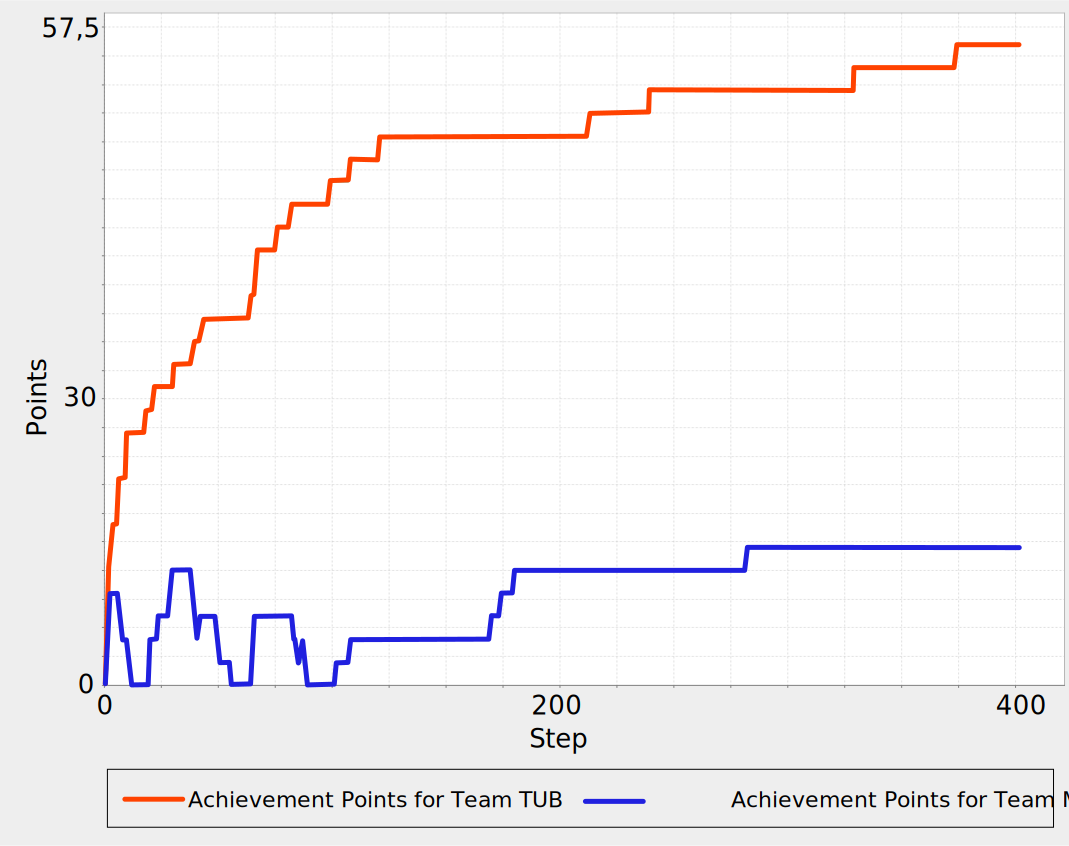
\includegraphics[width=300px]{images/AchievementPoints.png}
	\caption{MAPC 2014 result}
	\label{dis:achievement_points}
\end{figure}
It looks like that this is a huge drawback because achievement points earned at some point count into every future step score. But compared to the number of points awarded for zones, this is only a minor fraction of the step score. As it can be seen in figure \autoref{dis:ZonesScoresAndAchievementPoints} the spending of achievement points paid off since our upgraded saboteur agents hindered the enemy agents from building high valued zones. It was worth spending the achievement points for the purpose of attacking and disturbing the other team because the amount of potential zone points they would have earned without being attacked, is probably much higher than the amount of achievement points team "MaKo" spent for upgrades.
\begin{figure}[h]
	\centering
	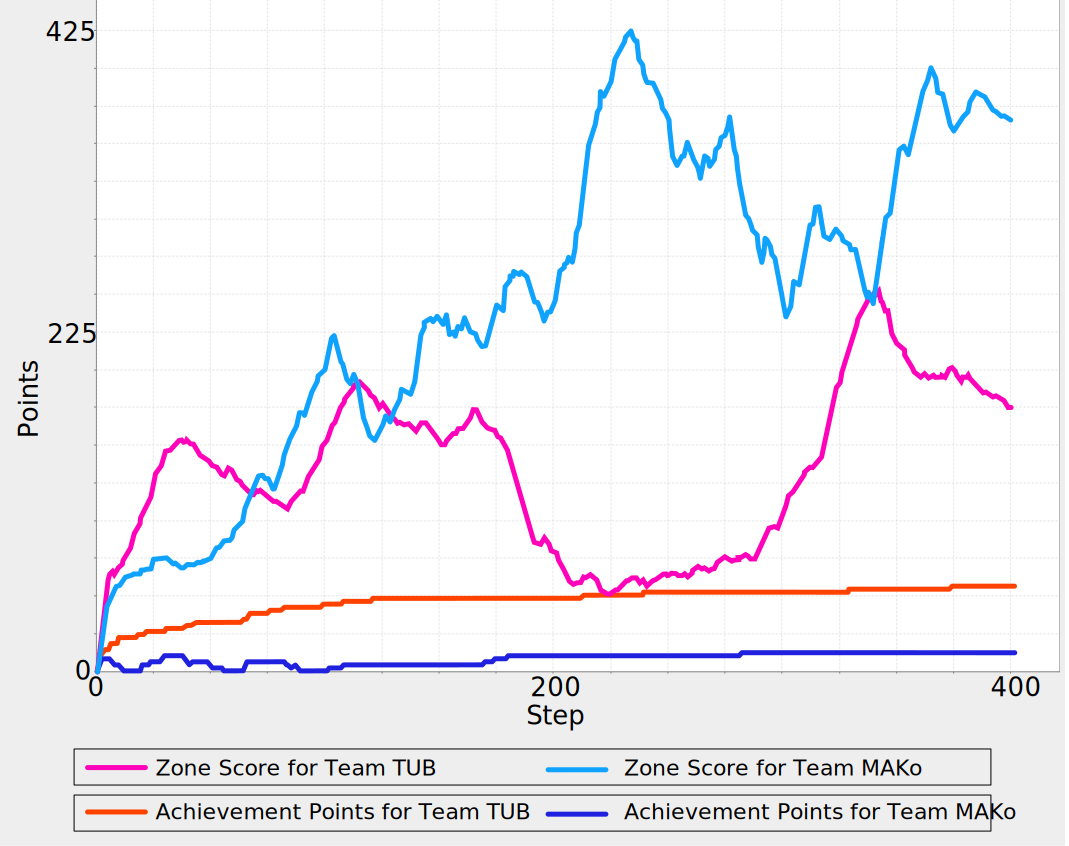
\includegraphics[width=300px]{images/ZonesScoresAndAchievementPoints.png}
	\caption{MAPC 2014 result}
	\label{dis:ZonesScoresAndAchievementPoints}
\end{figure}
At the end of the tournament team "MaKo" scored second with a total of 18 points. The winner 2014 was, for three times in a row now, the team from the USFC. The final results are shown in~\autoref{tab:mapc2014results}.
\begin{table}[ht]
\centering
\caption{The results of the 2014 MAPC. Each team played three matches against every other team, and winning a match awarded 3 points.}
\label{tab:mapc2014results}
\begin{tabular}{@{}lllll@{}}
\toprule
Pos. & Team name      & Score            & Difference            & Points \\ \midrule
1    & SMADAS-UFSC    & 1180662 : 654624 & \phantom{-}526038     & 33     \\
2    & MAKo           & 617086 : 776868  & -15782                & 18     \\
3    & TUB            & 904874 : 872399  & \phantom{-}32475      & 15     \\
4    & TheWonderbolts & 711001 : 1014669 & -303668               & 15     \\
5    & GOAL-DTU       & 653178 : 748241  & -95063                & 9      \\ \bottomrule
\end{tabular}
\end{table}
Statistics of all the individual games can be found in the appendix.[reference here!!!!]

Team "MaKo" lost every second game against each opponent due to the fact that for some reason the repairer agents weren't able to repair. The reason behind this was not obvious to the team. Summarizing the matches, team "MaKo" was capable of exploring the map, building local optima zones, dealing with disabled agents and attacking the opponent. A thing that could be improved is the zoning behaviour. Due to the fact that zones were broken up on a regular basis, zones with a high value sometimes were discarded even when there was no need to do that. Also no handling of edge cases has been implemented which could improve zoning in the sense that the actual number of agents needed to build that zone could be less than the number calculated by our algorithm. But the general idea regarding small zone forming was good. Because one big zone is easy to disturb, having some small high value zones was quite effective to not provide the enemy with an easy target. Like already mentioned a strategy that worked out well, was the approach to upgrade the visibility range and the strength of one saboteur agent significantly. In all matches the it was able to disable enemy agents many times and therefore disturb zones and keep the enemy repairers busy, which kept them away from building zones. 

% TODO: these are from the TOC:
%What place did we rank? How did the others do? Analyse our matches shortly and point out problems we faced, how we tackled them and point out what had gone well.


\subsection{Lessons learned$^{\odot}$}
None of the "MaKo" team member had experience with Jason as a programming language before the research lab.
The first thing that caused problems was that Jason was quite slow, especially when it comes to communication between agents.
Since agents most times needed some information from others and could not continue with their reasoning until this information was given, communication was a extreme bottleneck.
Extreme delay was observed when the group tried to exchange information about the graph.
The first approach was to communicate everything that an agent perceives, while exploring the graph, to every other agent.
The reason behind this was to have every agent store the full knowledge about the until then explored (sub-)graph.
This course of action was quickly discarded, because agents were not able to do actions while processing all the incoming messages.
The next attempt to reduce communication was to implement a so called "cartographer" agent.
The purpose of this agent was to have an additionally agent in the background that gathers all the information about the map that all 28 agents perceive.
With that cartographer agent the amount of communication was reduced and agents could act like intended, because now they just sent their percepts to the cartographer agent and they had not to deal with incoming messages of the other 27 agents.
The drawback of this approach revealed when it came to querying the cartographer agent for information, for instance when an agent wanted to know if a vertex was already surveyed or how he could reach given vertex.
Like it was noticed before, processing the received messages is quite slow and so it happened that the cartographer agent was not able to handle messages in time.
It occurred that agents asked about some specific vertex which the cartographer agent should have known about (because some other agent already informed him about that particular vertex) and they got no answer due to the fact that the cartographer agent hadn't processed the message yet.
That's why this approach was also discarded.
The next idea, which worked in the end, was to use a Java object, the so called "map agent", for the purpose of storing and processing graph information.
Internal actions were used to obtain the required information about the graph.
For instance the internal action "getBestHopToVertex" calculates the shortest path and returns, for a given target node, the next vertex where the agent has to go to.
Another issue that arose initially during the contest was that if a Term in Jason contains a dash, it is interpreted as a Number.
We observed this during our first match against a team that had a dash in its name.
The result was that we were not able to distinguish between friendly and enemy agents.
We immediately fixed it, so that in the next matches we took this possibility of having a dash in the team name into account.

% TODO: these are from the TOC
%Here we could explain what was working well and what was troublesome.  Java: fast.  AS(L): slow and hard for us to program.  Communication: extreme bottleneck.  Also we could note that all this would need much more time and preparation (or a team that is more familiar with agent programming).  %We can illustrate this with our approaches of a dedicated cartographer agent and the node agents.  We might also illustrate further failed approaches.



%\bibliographystyle{../tech_reports/template/splncs03}
%\clearpage
%\bibliography{./content/sources}
\printbibliography
\end{document}
